\documentclass[12pt,brazil,oneside]{book}
\usepackage{lmodern}
\usepackage{amssymb,amsmath}
\usepackage{ifxetex,ifluatex}
\usepackage{fixltx2e} % provides \textsubscript
\ifnum 0\ifxetex 1\fi\ifluatex 1\fi=0 % if pdftex
  \usepackage[T1]{fontenc}
  \usepackage[utf8]{inputenc}
\else % if luatex or xelatex
  \ifxetex
    \usepackage{mathspec}
  \else
    \usepackage{fontspec}
  \fi
  \defaultfontfeatures{Ligatures=TeX,Scale=MatchLowercase}
\fi
% use upquote if available, for straight quotes in verbatim environments
\IfFileExists{upquote.sty}{\usepackage{upquote}}{}
% use microtype if available
\IfFileExists{microtype.sty}{%
\usepackage{microtype}
\UseMicrotypeSet[protrusion]{basicmath} % disable protrusion for tt fonts
}{}
\usepackage[margin=1in]{geometry}
\usepackage{hyperref}
\hypersetup{unicode=true,
            pdftitle={Software R: curso avançado},
            pdfauthor={Felipe Micail da Silva Smolski; Iara Denise Endruweit Battisti},
            pdfborder={0 0 0},
            breaklinks=true}
\urlstyle{same}  % don't use monospace font for urls
\ifnum 0\ifxetex 1\fi\ifluatex 1\fi=0 % if pdftex
  \usepackage[shorthands=off,main=brazil]{babel}
\else
  \usepackage{polyglossia}
  \setmainlanguage[]{brazil}
\fi
\usepackage{color}
\usepackage{fancyvrb}
\newcommand{\VerbBar}{|}
\newcommand{\VERB}{\Verb[commandchars=\\\{\}]}
\DefineVerbatimEnvironment{Highlighting}{Verbatim}{commandchars=\\\{\}}
% Add ',fontsize=\small' for more characters per line
\usepackage{framed}
\definecolor{shadecolor}{RGB}{248,248,248}
\newenvironment{Shaded}{\begin{snugshade}}{\end{snugshade}}
\newcommand{\AlertTok}[1]{\textcolor[rgb]{0.94,0.16,0.16}{#1}}
\newcommand{\AnnotationTok}[1]{\textcolor[rgb]{0.56,0.35,0.01}{\textbf{\textit{#1}}}}
\newcommand{\AttributeTok}[1]{\textcolor[rgb]{0.77,0.63,0.00}{#1}}
\newcommand{\BaseNTok}[1]{\textcolor[rgb]{0.00,0.00,0.81}{#1}}
\newcommand{\BuiltInTok}[1]{#1}
\newcommand{\CharTok}[1]{\textcolor[rgb]{0.31,0.60,0.02}{#1}}
\newcommand{\CommentTok}[1]{\textcolor[rgb]{0.56,0.35,0.01}{\textit{#1}}}
\newcommand{\CommentVarTok}[1]{\textcolor[rgb]{0.56,0.35,0.01}{\textbf{\textit{#1}}}}
\newcommand{\ConstantTok}[1]{\textcolor[rgb]{0.00,0.00,0.00}{#1}}
\newcommand{\ControlFlowTok}[1]{\textcolor[rgb]{0.13,0.29,0.53}{\textbf{#1}}}
\newcommand{\DataTypeTok}[1]{\textcolor[rgb]{0.13,0.29,0.53}{#1}}
\newcommand{\DecValTok}[1]{\textcolor[rgb]{0.00,0.00,0.81}{#1}}
\newcommand{\DocumentationTok}[1]{\textcolor[rgb]{0.56,0.35,0.01}{\textbf{\textit{#1}}}}
\newcommand{\ErrorTok}[1]{\textcolor[rgb]{0.64,0.00,0.00}{\textbf{#1}}}
\newcommand{\ExtensionTok}[1]{#1}
\newcommand{\FloatTok}[1]{\textcolor[rgb]{0.00,0.00,0.81}{#1}}
\newcommand{\FunctionTok}[1]{\textcolor[rgb]{0.00,0.00,0.00}{#1}}
\newcommand{\ImportTok}[1]{#1}
\newcommand{\InformationTok}[1]{\textcolor[rgb]{0.56,0.35,0.01}{\textbf{\textit{#1}}}}
\newcommand{\KeywordTok}[1]{\textcolor[rgb]{0.13,0.29,0.53}{\textbf{#1}}}
\newcommand{\NormalTok}[1]{#1}
\newcommand{\OperatorTok}[1]{\textcolor[rgb]{0.81,0.36,0.00}{\textbf{#1}}}
\newcommand{\OtherTok}[1]{\textcolor[rgb]{0.56,0.35,0.01}{#1}}
\newcommand{\PreprocessorTok}[1]{\textcolor[rgb]{0.56,0.35,0.01}{\textit{#1}}}
\newcommand{\RegionMarkerTok}[1]{#1}
\newcommand{\SpecialCharTok}[1]{\textcolor[rgb]{0.00,0.00,0.00}{#1}}
\newcommand{\SpecialStringTok}[1]{\textcolor[rgb]{0.31,0.60,0.02}{#1}}
\newcommand{\StringTok}[1]{\textcolor[rgb]{0.31,0.60,0.02}{#1}}
\newcommand{\VariableTok}[1]{\textcolor[rgb]{0.00,0.00,0.00}{#1}}
\newcommand{\VerbatimStringTok}[1]{\textcolor[rgb]{0.31,0.60,0.02}{#1}}
\newcommand{\WarningTok}[1]{\textcolor[rgb]{0.56,0.35,0.01}{\textbf{\textit{#1}}}}
\usepackage{longtable,booktabs}
\usepackage{graphicx,grffile}
\makeatletter
\def\maxwidth{\ifdim\Gin@nat@width>\linewidth\linewidth\else\Gin@nat@width\fi}
\def\maxheight{\ifdim\Gin@nat@height>\textheight\textheight\else\Gin@nat@height\fi}
\makeatother
% Scale images if necessary, so that they will not overflow the page
% margins by default, and it is still possible to overwrite the defaults
% using explicit options in \includegraphics[width, height, ...]{}
\setkeys{Gin}{width=\maxwidth,height=\maxheight,keepaspectratio}
\IfFileExists{parskip.sty}{%
\usepackage{parskip}
}{% else
\setlength{\parindent}{0pt}
\setlength{\parskip}{6pt plus 2pt minus 1pt}
}
\setlength{\emergencystretch}{3em}  % prevent overfull lines
\providecommand{\tightlist}{%
  \setlength{\itemsep}{0pt}\setlength{\parskip}{0pt}}
\setcounter{secnumdepth}{5}
% Redefines (sub)paragraphs to behave more like sections
\ifx\paragraph\undefined\else
\let\oldparagraph\paragraph
\renewcommand{\paragraph}[1]{\oldparagraph{#1}\mbox{}}
\fi
\ifx\subparagraph\undefined\else
\let\oldsubparagraph\subparagraph
\renewcommand{\subparagraph}[1]{\oldsubparagraph{#1}\mbox{}}
\fi

%%% Use protect on footnotes to avoid problems with footnotes in titles
\let\rmarkdownfootnote\footnote%
\def\footnote{\protect\rmarkdownfootnote}

%%% Change title format to be more compact
\usepackage{titling}

% Create subtitle command for use in maketitle
\newcommand{\subtitle}[1]{
  \posttitle{
    \begin{center}\large#1\end{center}
    }
}

\setlength{\droptitle}{-2em}

  \title{Software R: curso avançado}
    \pretitle{\vspace{\droptitle}\centering\huge}
  \posttitle{\par}
    \author{Felipe Micail da Silva Smolski \\ Iara Denise Endruweit Battisti}
    \preauthor{\centering\large\emph}
  \postauthor{\par}
      \predate{\centering\large\emph}
  \postdate{\par}
    \date{2018-08-05}

\usepackage{booktabs}
\usepackage{multirow}
\usepackage{longtable,ltcaption}
\usepackage{pdfpages}
\usepackage[T1]{fontenc}		% Selecao de codigos de fonte.
\usepackage[utf8]{inputenc}		% Codificacao do documento (conversão automática dos acentos)
\usepackage{lastpage}			% Usado pela Ficha catalográfica
\usepackage{indentfirst}		% Indenta o primeiro parágrafo de cada seção.
\usepackage{color}				% Controle das cores
\usepackage{graphicx}

\setlength{\parskip}{1em}
\renewcommand{\baselinestretch}{1.0}
\setlength{\parindent}{1.25cm}
\selectlanguage{brazil}

\begin{document}
\maketitle

{
\setcounter{tocdepth}{1}
\tableofcontents
}
\hypertarget{prefacio}{%
\chapter*{Prefácio}\label{prefacio}}
\addcontentsline{toc}{chapter}{Prefácio}

Esta é a estrutura provisória de capítulos do \textbf{Curso Avançado em
Estatística com R da UFFS}:

\begin{itemize}
\tightlist
\item
  Delineamentos Experimentais
\item
  Análise Fatorial
\item
  Regressão Múltipla
\item
  Regressão Logística
\end{itemize}

Algumas sugestões a incluir:

\begin{itemize}
\tightlist
\item
  Produção de Mapas
\item
  Análise de Clusters
\item
  Manipulação de bases de dados
\item
  Análise de redes
\item
  O que mais?
\end{itemize}


\includegraphics{Capa1.png}

\hypertarget{introducao}{%
\chapter*{Introdução}\label{introducao}}
\addcontentsline{toc}{chapter}{Introdução}

\hypertarget{delineamentos-experimentais}{%
\chapter{Delineamentos
Experimentais}\label{delineamentos-experimentais}}

A experimentação é uma parte da estatística probabilística que estuda o
planejamento, execução, coleta de dados, análise de dados e
interpretação dos resultados provenientes de um experimento.

Um experimento é um procedimento planejado com base em uma hipótese, que
tem por objetivo provocar fenômenos (tratamentos) de forma controlada,
analisando e interpretando os resultados obtidos.

O tratamento é o método, elemento ou material cujo efeito desejamos
avaliar em um experimento. Por exemplo: formas de preparo de solo,
diferentes cultivares, doses de adubação, controle de insetos e outras
pragas, controle de uma doença. Num experimento, somente o tratamento
variade uma unidade experimental para outra, as demais condições são
mantidas constantes, salvo erros não controláveis.

E alguns experimentos, utiliza-se a testemunha (nas ciências agrárias e
ambientais) ou placebo (na saúde), que são as unidades experimentais que
não recebem tratamento.

A unidade experimental é a unidade que recebe o tratamento uma vez e,
normalmente são chamadas de parcelas. A escolha da unidade experimental
depende dos tipos de tratamentos que serão avaliados. Podem ser: uma
área de campo, um vaso com solo, um animal, uma placa de Petri, uma
planta. Em áreas de campo, normalmente utiliza-se a bordadura. Num
experimento, recomenda-se, no mínimo, a utilização de 20 UEs.

Em um experimento, a variável a ser avaliada chamamos de variável
resposta. Por exemplo, núumero de grãos por planta, número de folhas por
planta, altura das plantas.

\hypertarget{principios-basicos-da-experimentacao}{%
\section{Princípios básicos da
Experimentação}\label{principios-basicos-da-experimentacao}}

\hypertarget{repeticao}{%
\subsection{Repetição}\label{repeticao}}

A repetição consiste na aplicação do mesmo tratamento sobre duas ou mais
unidades experimentais. Permite estimar o erro experimental e avaliar de
forma mais precisa o efeito de cada tratamento.

O erro experimental é caracterizado pela variância entre as unidades
experimentais que receberam o mesmo tratamento.

\hypertarget{casualizacao}{%
\subsection{Casualização}\label{casualizacao}}

A casualização consiste na aplicação dos tratamentos aleatoriamente
(sorteio) sobre as unidades experimentais. A casualização é usada para
obter a independência dos erros, ou seja, evitar que determinados
tratamentos sejam favorecidos.

\hypertarget{controle-local}{%
\subsection{Controle local}\label{controle-local}}

Quando tiver heterogeneidade no material experimental: plantas de
diferentes alturas, animais de diferentes idades, solo com declividade,
deve-se separar o material em grupos homogêneos e aplicar o tratamento
uma vez dentro de cada grupo (blocos). A homogeneidade ou não do
material dá origem aos tipos de delineamentos:

\begin{itemize}
\item
  Delineamento Inteiramente Casualizado (DIC): material experimental
  homogêneo;
\item
  Delineamento Blocos Casualizados (DBC): material experimental com uma
  fonte de heterogeneidade;
\item
  Delineamento Quadrado Latino (DQL): material experimental com duas
  fontes de heterogeneidade.
\end{itemize}

\hypertarget{analise-de-variancia}{%
\section{Análise de Variância}\label{analise-de-variancia}}

Para saber se existe diferença significativa entre as médias resultados
dos efeitos de tratamentos, realiza-se a Análise de Variância (ANOVA).

\begin{longtable}[]{@{}cccccc@{}}
\caption{Nome da Tabela}\tabularnewline
\toprule
\begin{minipage}[b]{0.14\columnwidth}\centering
\textbf{Fonte de Variação}\strut
\end{minipage} & \begin{minipage}[b]{0.14\columnwidth}\centering
\textbf{Graus de Liberdade (GL)}\strut
\end{minipage} & \begin{minipage}[b]{0.14\columnwidth}\centering
\textbf{Soma de Quadrados (SQ)}\strut
\end{minipage} & \begin{minipage}[b]{0.14\columnwidth}\centering
\textbf{Quadrado Médio (QM)}\strut
\end{minipage} & \begin{minipage}[b]{0.14\columnwidth}\centering
\textbf{Falc}\strut
\end{minipage} & \begin{minipage}[b]{0.14\columnwidth}\centering
\textbf{P}\strut
\end{minipage}\tabularnewline
\midrule
\endfirsthead
\toprule
\begin{minipage}[b]{0.14\columnwidth}\centering
\textbf{Fonte de Variação}\strut
\end{minipage} & \begin{minipage}[b]{0.14\columnwidth}\centering
\textbf{Graus de Liberdade (GL)}\strut
\end{minipage} & \begin{minipage}[b]{0.14\columnwidth}\centering
\textbf{Soma de Quadrados (SQ)}\strut
\end{minipage} & \begin{minipage}[b]{0.14\columnwidth}\centering
\textbf{Quadrado Médio (QM)}\strut
\end{minipage} & \begin{minipage}[b]{0.14\columnwidth}\centering
\textbf{Falc}\strut
\end{minipage} & \begin{minipage}[b]{0.14\columnwidth}\centering
\textbf{P}\strut
\end{minipage}\tabularnewline
\midrule
\endhead
\begin{minipage}[t]{0.14\columnwidth}\centering
Tratamento\strut
\end{minipage} & \begin{minipage}[t]{0.14\columnwidth}\centering
I-1\strut
\end{minipage} & \begin{minipage}[t]{0.14\columnwidth}\centering
SQtrat\strut
\end{minipage} & \begin{minipage}[t]{0.14\columnwidth}\centering
QMat\strut
\end{minipage} & \begin{minipage}[t]{0.14\columnwidth}\centering
QMatr/QMerro\strut
\end{minipage} & \begin{minipage}[t]{0.14\columnwidth}\centering
P\strut
\end{minipage}\tabularnewline
\begin{minipage}[t]{0.14\columnwidth}\centering
Erro\strut
\end{minipage} & \begin{minipage}[t]{0.14\columnwidth}\centering
GLerro\strut
\end{minipage} & \begin{minipage}[t]{0.14\columnwidth}\centering
SQerro\strut
\end{minipage} & \begin{minipage}[t]{0.14\columnwidth}\centering
QMerro\strut
\end{minipage} & \begin{minipage}[t]{0.14\columnwidth}\centering
\strut
\end{minipage} & \begin{minipage}[t]{0.14\columnwidth}\centering
\strut
\end{minipage}\tabularnewline
\begin{minipage}[t]{0.14\columnwidth}\centering
Total\strut
\end{minipage} & \begin{minipage}[t]{0.14\columnwidth}\centering
IJ-1\strut
\end{minipage} & \begin{minipage}[t]{0.14\columnwidth}\centering
SQtotal\strut
\end{minipage} & \begin{minipage}[t]{0.14\columnwidth}\centering
\strut
\end{minipage} & \begin{minipage}[t]{0.14\columnwidth}\centering
\strut
\end{minipage} & \begin{minipage}[t]{0.14\columnwidth}\centering
\strut
\end{minipage}\tabularnewline
\bottomrule
\end{longtable}

\hypertarget{hipoteses-estatisticas}{%
\section{Hipóteses estatísticas}\label{hipoteses-estatisticas}}

\begin{itemize}
\item
  H0: Não existe diferença entre as médias dos tratamentos
\item
  H1: Existe, pelo menos, uma diferença entre as médias dos tratamentos
\end{itemize}

\hypertarget{delineamento-inteiramente-causalizado-dic}{%
\section{Delineamento Inteiramente Causalizado
(DIC)}\label{delineamento-inteiramente-causalizado-dic}}

É utilizado quando as unidades experimentais são homogêneas. É o mais
simples dos delineamentos e os tratamentos são designados às unidades
experimentais de forma casualizada, por meio de um único sorteio. Usado
principalmente em pequenos animais, casas de vegetação e em
laboratórios.

\emph{Exemplo}: Um produtor deseja avaliar 4 variedades de pera (A, B, C
e D). Para tanto, instalou um experimento no delineamento inteiramente
casualizado, utilizando 5 repetições por variedade. Os resultados, peso
médio do fruto, estão apresentados a seguir:

\begin{figure}
\centering
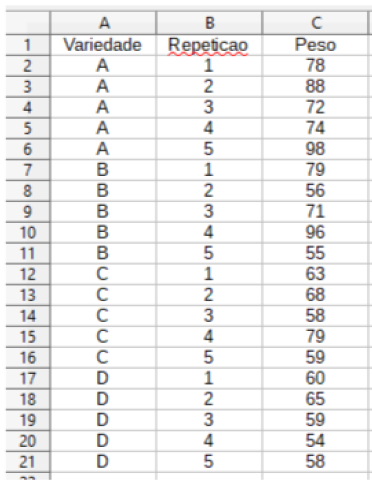
\includegraphics{delimexp0.png}
\caption{Variedades de pera separadas por grupos em faixas de peso e
repetição}
\end{figure}

Existe diferença significativa entre as variedades de pera, considerando
o peso médio dos frutos de cada variedade?

Para responder esta pergunta, utilizamos a Análise de Variância (ANOVA).

No software RStudio:

Criar o arquivo acima em planilha eletrônica. Nomear como DIC e salvar
em formato .xls.

Importar no RStudio:

\begin{Shaded}
\begin{Highlighting}[]
\KeywordTok{require}\NormalTok{(readxl)}
\NormalTok{url <-}\StringTok{ "https://github.com/Smolski/softwarelivrer/raw/master/avancado/dic.xls"}
\NormalTok{destfile <-}\StringTok{ "dic.xls"}
\NormalTok{curl}\OperatorTok{::}\KeywordTok{curl_download}\NormalTok{(url, destfile)}
\NormalTok{DIC <-}\StringTok{ }\KeywordTok{read_excel}\NormalTok{(destfile)}
\KeywordTok{attach}\NormalTok{(DIC)}
\end{Highlighting}
\end{Shaded}

O comando que gera a análise de variância é o \texttt{aov()} e o comando
que exibe o quadro da ANOVA é o \texttt{anova}. Então, podemos gerar o
quadro da análise de uma são vez associando os dois comandos.

\begin{Shaded}
\begin{Highlighting}[]
\NormalTok{anova=}\KeywordTok{aov}\NormalTok{(Peso}\OperatorTok{~}\NormalTok{Variedade)}
\KeywordTok{summary}\NormalTok{(anova)}
\end{Highlighting}
\end{Shaded}

\begin{verbatim}
            Df Sum Sq Mean Sq F value Pr(>F)  
Variedade    3   1414     471    3.78  0.032 *
Residuals   16   1997     125                 
---
Signif. codes:  0 '***' 0.001 '**' 0.01 '*' 0.05 '.' 0.1 ' ' 1
\end{verbatim}

Hipóteses estatísticas:

\begin{itemize}
\tightlist
\item
  H0: ti \(=\) 0 (as médias dos tratamentos nãao diferem entre si)
\item
  H1: ti \(\neq\) 0 (existe, no mínimo, uma diferença entre as médias
  dos tratamentos)
\end{itemize}

Como p = 0,0319 (0,01 \(\leq\) p ``menor ou igual a'' 0,05), rejeita-se
H0 com nível de significância de 5\% e conclui-se que existe diferença
significativa entre as médias dos tratamentos.

Para saber quais as médias que diferem, utilizamos o teste de Tukey.

\begin{Shaded}
\begin{Highlighting}[]
\KeywordTok{attach}\NormalTok{(DIC)}
\end{Highlighting}
\end{Shaded}

\begin{verbatim}
The following objects are masked from DIC (pos = 3):

    Peso, Repeticao, Variedade
\end{verbatim}

\begin{Shaded}
\begin{Highlighting}[]
\KeywordTok{TukeyHSD}\NormalTok{(anova,}\KeywordTok{as.factor}\NormalTok{(}\StringTok{"Variedade"}\NormalTok{),}\DataTypeTok{ordered=}\OtherTok{TRUE}\NormalTok{)}
\end{Highlighting}
\end{Shaded}

\begin{verbatim}
  Tukey multiple comparisons of means
    95% family-wise confidence level
    factor levels have been ordered

Fit: aov(formula = Peso ~ Variedade)

$Variedade
    diff     lwr   upr  p adj
C-D  6.2 -14.016 26.42 0.8164
B-D 12.2  -8.016 32.42 0.3429
A-D 22.8   2.584 43.02 0.0245
B-C  6.0 -14.216 26.22 0.8303
A-C 16.6  -3.616 36.82 0.1282
A-B 10.6  -9.616 30.82 0.4602
\end{verbatim}

Para que o RStudio apresente uma tabela com as médias e letras indicando
quais as médias que diferiram, devemos instalar o pacote
\texttt{agricolae}.

\begin{Shaded}
\begin{Highlighting}[]
\KeywordTok{library}\NormalTok{(agricolae)}
\KeywordTok{HSD.test}\NormalTok{(anova,}\KeywordTok{as.factor}\NormalTok{(}\StringTok{"Variedade"}\NormalTok{),}\DataTypeTok{console=}\OtherTok{TRUE}\NormalTok{)}
\end{Highlighting}
\end{Shaded}

\begin{verbatim}

Study: anova ~ as.factor("Variedade")

HSD Test for Peso 

Mean Square Error:  124.8 

Variedade,  means

  Peso    std r Min Max
A 82.0 10.863 5  72  98
B 71.4 17.097 5  55  96
C 65.4  8.562 5  58  79
D 59.2  3.962 5  54  65

Alpha: 0.05 ; DF Error: 16 
Critical Value of Studentized Range: 4.046 

Minimun Significant Difference: 20.22 

Treatments with the same letter are not significantly different.

  Peso groups
A 82.0      a
B 71.4     ab
C 65.4     ab
D 59.2      b
\end{verbatim}

*Médias dos tratamentos não seguidas por mesma letra diferem pelo teste
de Tukey, ao nível de 5\% de significância.

Conclusão: A variedade de pera A apresentou o maior peso médio dos
frutos, que não diferiu significativamente do peso médio das variedades
B e C. A variedade de pera D apresentou o menor peso médio dos frutos,
que não diferiu significativamente do peso médio das variedades B e C.
As variedades B e C apresentaram peso médio dos frutos intermediário.

\begin{Shaded}
\begin{Highlighting}[]
\KeywordTok{attach}\NormalTok{(DIC)}
\end{Highlighting}
\end{Shaded}

\begin{verbatim}
The following objects are masked from DIC (pos = 4):

    Peso, Repeticao, Variedade
\end{verbatim}

\begin{verbatim}
The following objects are masked from DIC (pos = 5):

    Peso, Repeticao, Variedade
\end{verbatim}

\begin{Shaded}
\begin{Highlighting}[]
\KeywordTok{boxplot}\NormalTok{(Peso}\OperatorTok{~}\NormalTok{Variedade)}
\KeywordTok{boxplot}\NormalTok{(Peso}\OperatorTok{~}\NormalTok{Variedade,}\DataTypeTok{xlab=}\StringTok{"Variedade"}\NormalTok{,}\DataTypeTok{ylab=}\StringTok{"Peso"}\NormalTok{)}
\end{Highlighting}
\end{Shaded}

\begin{center}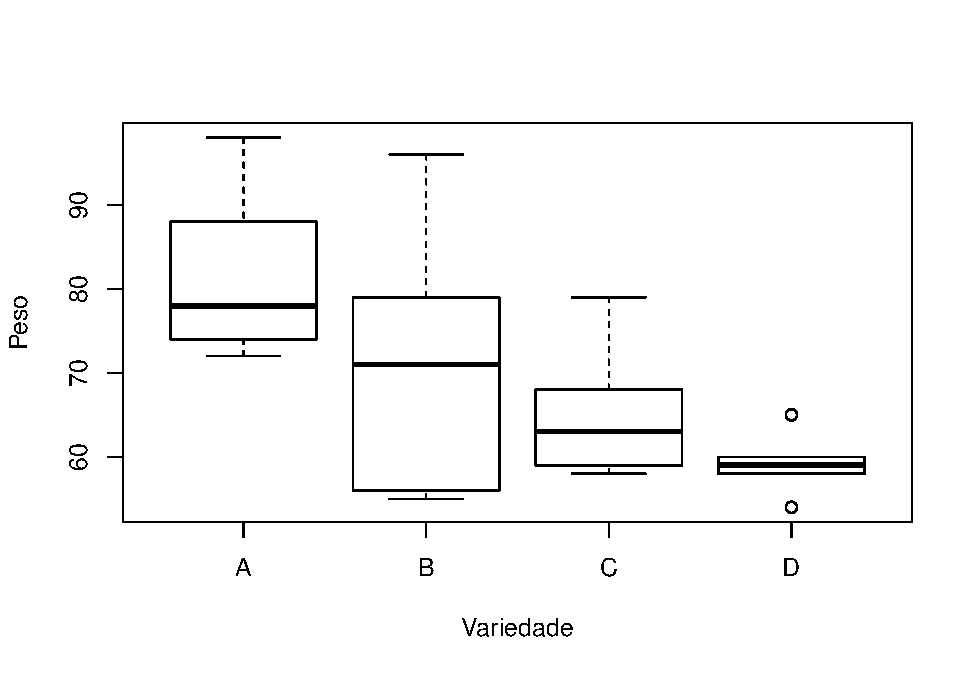
\includegraphics[width=0.6\linewidth]{02-Delinexp_files/figure-latex/unnamed-chunk-6-1} \end{center}

\begin{Shaded}
\begin{Highlighting}[]
\KeywordTok{tapply}\NormalTok{(Peso,Variedade,mean)}
\end{Highlighting}
\end{Shaded}

\begin{verbatim}
   A    B    C    D 
82.0 71.4 65.4 59.2 
\end{verbatim}

\begin{Shaded}
\begin{Highlighting}[]
\KeywordTok{tapply}\NormalTok{(Peso,Variedade,sd)}
\end{Highlighting}
\end{Shaded}

\begin{verbatim}
     A      B      C      D 
10.863 17.097  8.562  3.962 
\end{verbatim}

\begin{Shaded}
\begin{Highlighting}[]
\NormalTok{residuos=}\KeywordTok{residuals}\NormalTok{(anova)}
\NormalTok{ajustados=}\KeywordTok{fitted}\NormalTok{(anova)}
\KeywordTok{plot}\NormalTok{(ajustados,residuos)}
\KeywordTok{abline}\NormalTok{(}\DataTypeTok{h=}\DecValTok{0}\NormalTok{)}
\end{Highlighting}
\end{Shaded}

\begin{center}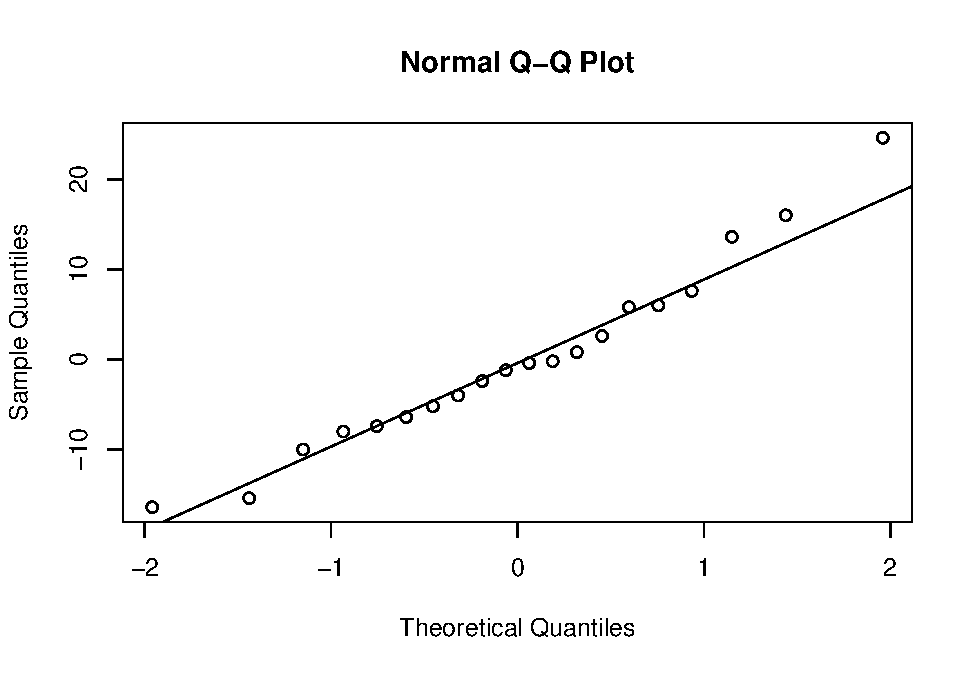
\includegraphics[width=0.6\linewidth]{02-Delinexp_files/figure-latex/unnamed-chunk-8-1} \end{center}

\begin{Shaded}
\begin{Highlighting}[]
\KeywordTok{qqnorm}\NormalTok{(residuos)}
\KeywordTok{qqline}\NormalTok{(residuos)}
\end{Highlighting}
\end{Shaded}

\begin{center}\includegraphics[width=0.6\linewidth]{02-Delinexp_files/figure-latex/unnamed-chunk-9-1} \end{center}

\hypertarget{delineamento-blocos-casualizados-dbc}{%
\section{Delineamento Blocos Casualizados
(DBC)}\label{delineamento-blocos-casualizados-dbc}}

É utilizado quando as unidades experimentais são heterogêneas. Os
tratamentos são designados às unidades experimentais de forma
casualizada, por meio de sorteio por blocos. Na área agrícola, é usado
principalmente em áreas de campo e grandes animais.

\emph{Exemplo}: Uma Nutricionista elaborou 4 dietas e quer aplicá-las em
20 pessoas a fim detestar suas eficiências quanto à perda de peso. Porém
ela notou que entre essas 20 pessoas existem 5 grupos de faixas iniciais
de peso. Então, para aumentar a eficácia do teste ela separou os 20
indivíduos em 5 grupos de faixas de peso.

\begin{figure}
\centering
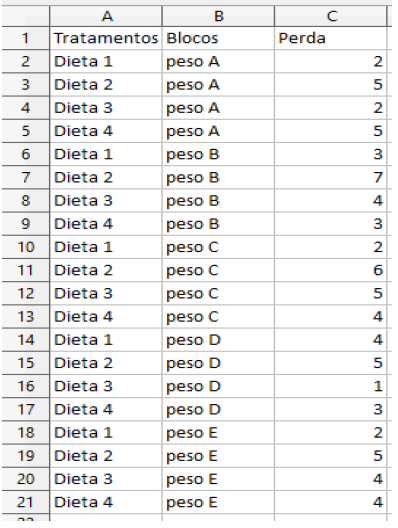
\includegraphics{delimexp1.png}
\caption{Indivíduos separados por grupos em faixas de peso}
\end{figure}

Criar o arquivo acima em planilha eletrônica. Nomear como DBC e salvar
em formato .xls.

Importar no RStudio:

\begin{Shaded}
\begin{Highlighting}[]
\KeywordTok{require}\NormalTok{(readxl)}
\NormalTok{url <-}\StringTok{ "https://github.com/Smolski/softwarelivrer/raw/master/avancado/dbc.xls"}
\NormalTok{destfile <-}\StringTok{ "dbc.xls"}
\NormalTok{curl}\OperatorTok{::}\KeywordTok{curl_download}\NormalTok{(url, destfile)}
\NormalTok{DBC  <-}\StringTok{ }\KeywordTok{read_excel}\NormalTok{(destfile)}

\KeywordTok{attach}\NormalTok{(DBC)}
\NormalTok{anova=}\KeywordTok{aov}\NormalTok{(Perda}\OperatorTok{~}\NormalTok{Tratamentos}\OperatorTok{+}\NormalTok{Blocos)}
\KeywordTok{summary}\NormalTok{(anova)}
\end{Highlighting}
\end{Shaded}

\begin{verbatim}
            Df Sum Sq Mean Sq F value Pr(>F)   
Tratamentos  3   25.2     8.4    6.00 0.0097 **
Blocos       4    3.2     0.8    0.57 0.6885   
Residuals   12   16.8     1.4                  
---
Signif. codes:  0 '***' 0.001 '**' 0.01 '*' 0.05 '.' 0.1 ' ' 1
\end{verbatim}

Hipóteses estatísticas:

\begin{itemize}
\tightlist
\item
  H0: ti \(=\) 0 (as médias dos tratamentos não diferem entre si)
\item
  H1: ti \(\neq\) 0 (existe, no mínimo, uma diferença entre as médias
  dos tratamentos)
\end{itemize}

Como p = 0,00973 (p \(\leq\) 0,01), rejeita-se H0 com nível de
significância de 1\% e conclui-se que existe diferença significativa
entre as médias dos tratamentos.

\begin{itemize}
\tightlist
\item
  H0: \(\sigma\)\textsuperscript{2} blocos \(=\) 0
\item
  H1: \(\sigma\)\textsuperscript{2} blocos \(\leq\) 0
\end{itemize}

Como p \(=\) 0,68854 (p \(\leq\) 0,05), não rejeita-se H0 e conclui-se
que a variância entre os blocos não é significativa.

\begin{Shaded}
\begin{Highlighting}[]
\KeywordTok{attach}\NormalTok{(DBC)}
\KeywordTok{HSD.test}\NormalTok{(anova,}\KeywordTok{as.factor}\NormalTok{(}\StringTok{"Tratamentos"}\NormalTok{),}\DataTypeTok{console=}\OtherTok{TRUE}\NormalTok{)}
\end{Highlighting}
\end{Shaded}

\begin{verbatim}

Study: anova ~ as.factor("Tratamentos")

HSD Test for Perda 

Mean Square Error:  1.4 

Tratamentos,  means

        Perda    std r Min Max
Dieta 1   2.6 0.8944 5   2   4
Dieta 2   5.6 0.8944 5   5   7
Dieta 3   3.2 1.6432 5   1   5
Dieta 4   3.8 0.8367 5   3   5

Alpha: 0.05 ; DF Error: 12 
Critical Value of Studentized Range: 4.199 

Minimun Significant Difference: 2.222 

Treatments with the same letter are not significantly different.

        Perda groups
Dieta 2   5.6      a
Dieta 4   3.8     ab
Dieta 3   3.2      b
Dieta 1   2.6      b
\end{verbatim}

Médias dos tratamentos não seguidas por mesma letra diferem pelo teste
de Tukey, ao nível de 5\% de significância.

Conclusão: A dieta que resultou na maior perda de peso foi a dieta 2,
que não diferiu da dieta 4. A dieta que resultou na menor perda de peso
foi a dieta 1, que não diferiu das dietas 3 e 4.

Medidas descritivas com a variável resposta:

\begin{Shaded}
\begin{Highlighting}[]
\KeywordTok{boxplot}\NormalTok{(Perda}\OperatorTok{~}\NormalTok{Tratamentos)}
\end{Highlighting}
\end{Shaded}

\begin{center}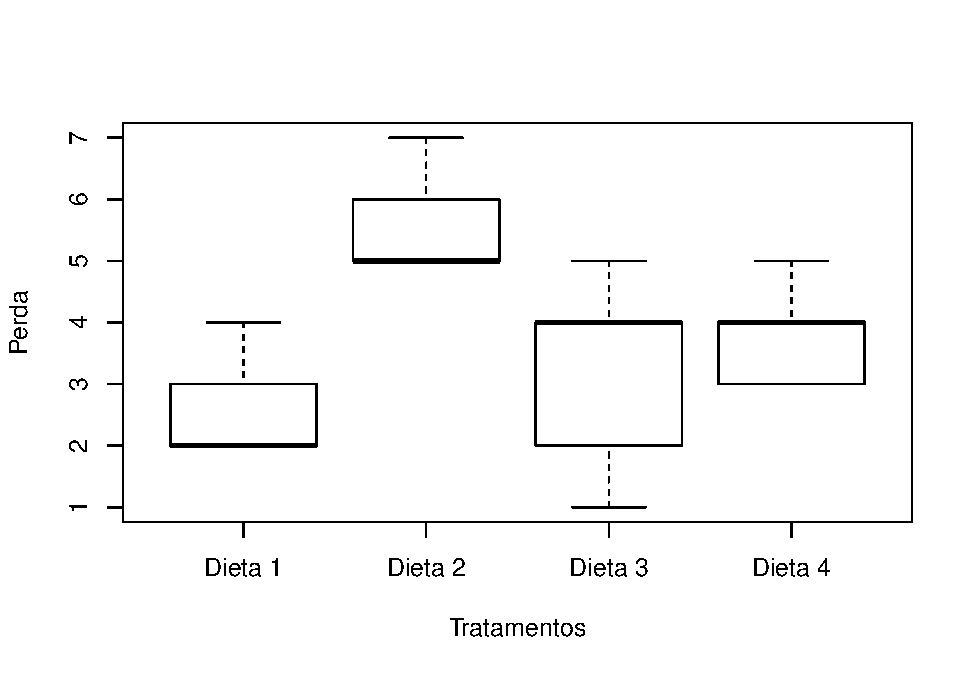
\includegraphics[width=0.6\linewidth]{02-Delinexp_files/figure-latex/unnamed-chunk-12-1} \end{center}

\begin{Shaded}
\begin{Highlighting}[]
\KeywordTok{boxplot}\NormalTok{(Perda}\OperatorTok{~}\NormalTok{Tratamentos,}\DataTypeTok{xlab=}\StringTok{"Tratamentos"}\NormalTok{,}\DataTypeTok{ylab=}\StringTok{"Perda"}\NormalTok{)}
\end{Highlighting}
\end{Shaded}

\begin{center}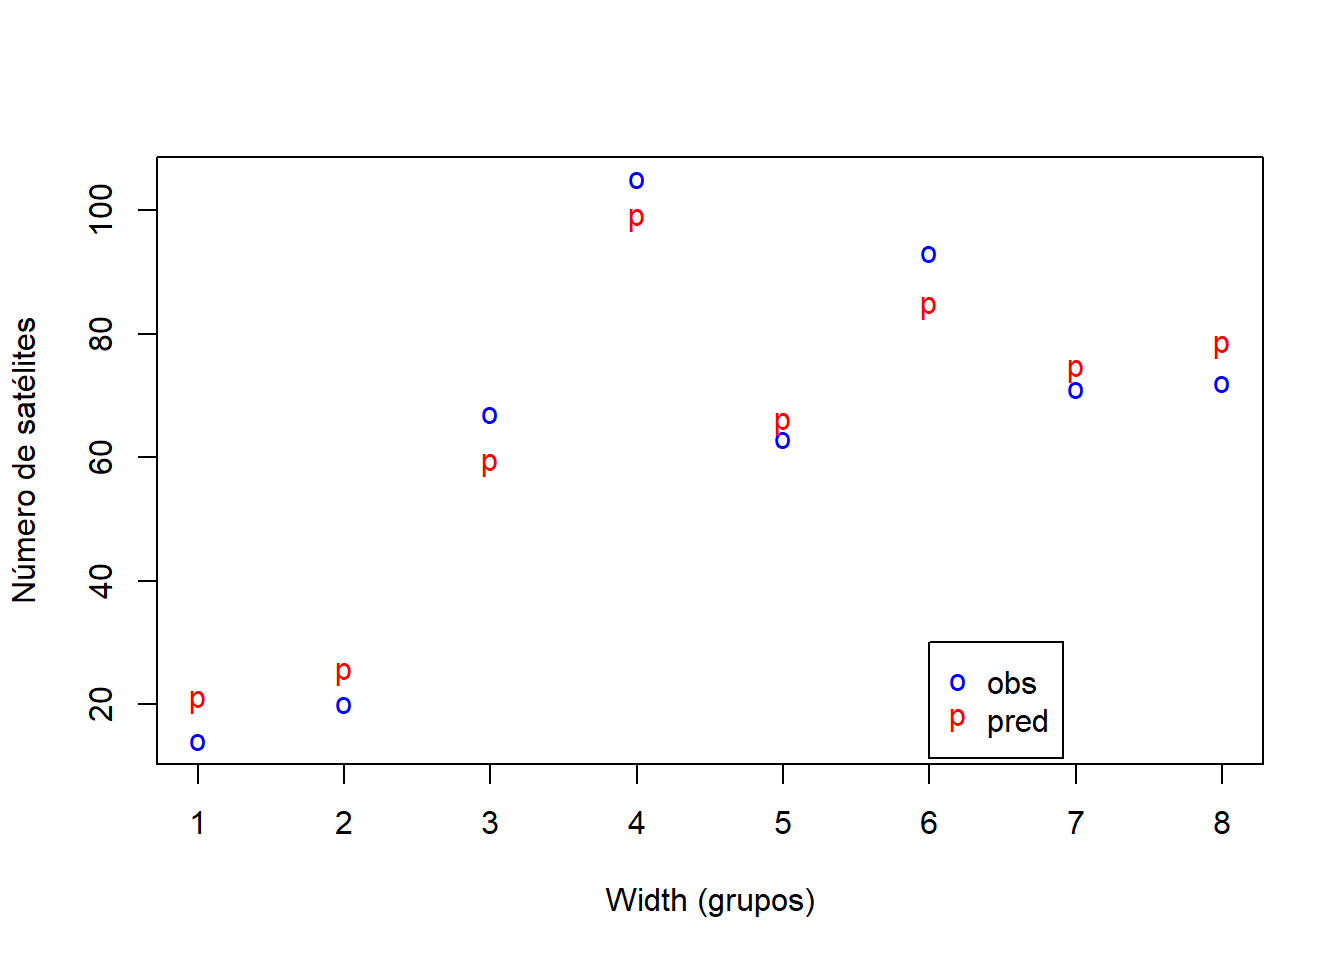
\includegraphics[width=0.6\linewidth]{02-Delinexp_files/figure-latex/unnamed-chunk-13-1} \end{center}

\begin{Shaded}
\begin{Highlighting}[]
\KeywordTok{tapply}\NormalTok{(Perda,Tratamentos,mean)}
\end{Highlighting}
\end{Shaded}

\begin{verbatim}
Dieta 1 Dieta 2 Dieta 3 Dieta 4 
    2.6     5.6     3.2     3.8 
\end{verbatim}

\begin{Shaded}
\begin{Highlighting}[]
\KeywordTok{tapply}\NormalTok{(Perda,Tratamentos,sd)}
\end{Highlighting}
\end{Shaded}

\begin{verbatim}
Dieta 1 Dieta 2 Dieta 3 Dieta 4 
 0.8944  0.8944  1.6432  0.8367 
\end{verbatim}

\begin{Shaded}
\begin{Highlighting}[]
\NormalTok{residuo=}\KeywordTok{residuals}\NormalTok{(anova)}
\NormalTok{ajustado=}\KeywordTok{fitted}\NormalTok{(anova)}
\KeywordTok{plot}\NormalTok{(ajustado,residuo)}
\KeywordTok{abline}\NormalTok{(}\DataTypeTok{h=}\DecValTok{0}\NormalTok{)}
\end{Highlighting}
\end{Shaded}

\begin{center}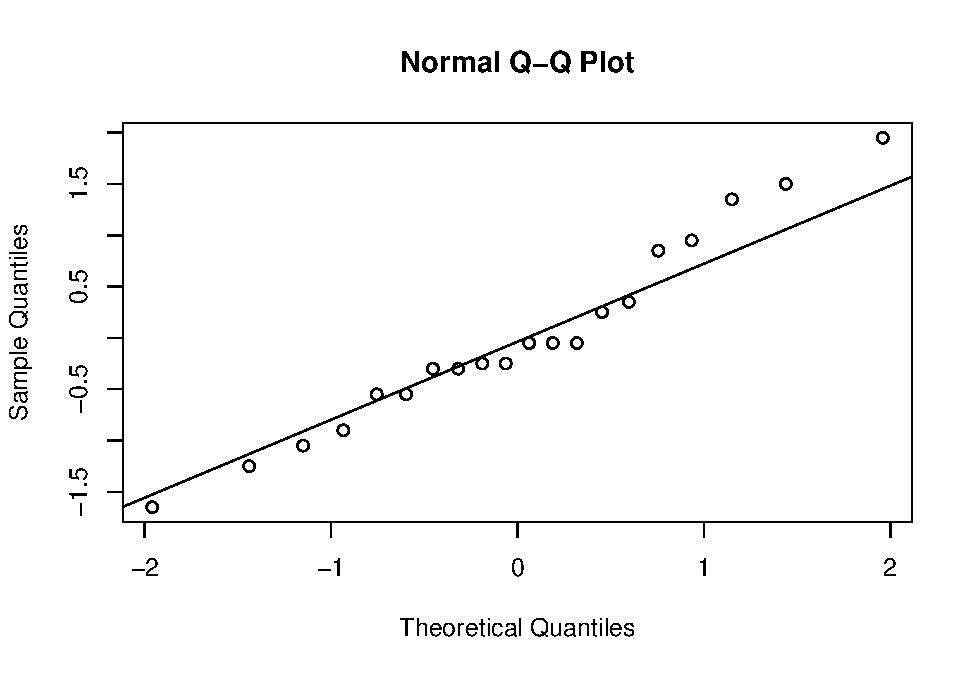
\includegraphics[width=0.6\linewidth]{02-Delinexp_files/figure-latex/unnamed-chunk-15-1} \end{center}

\begin{Shaded}
\begin{Highlighting}[]
\KeywordTok{qqnorm}\NormalTok{(residuo)}
\KeywordTok{qqline}\NormalTok{(residuo)}
\end{Highlighting}
\end{Shaded}

\begin{center}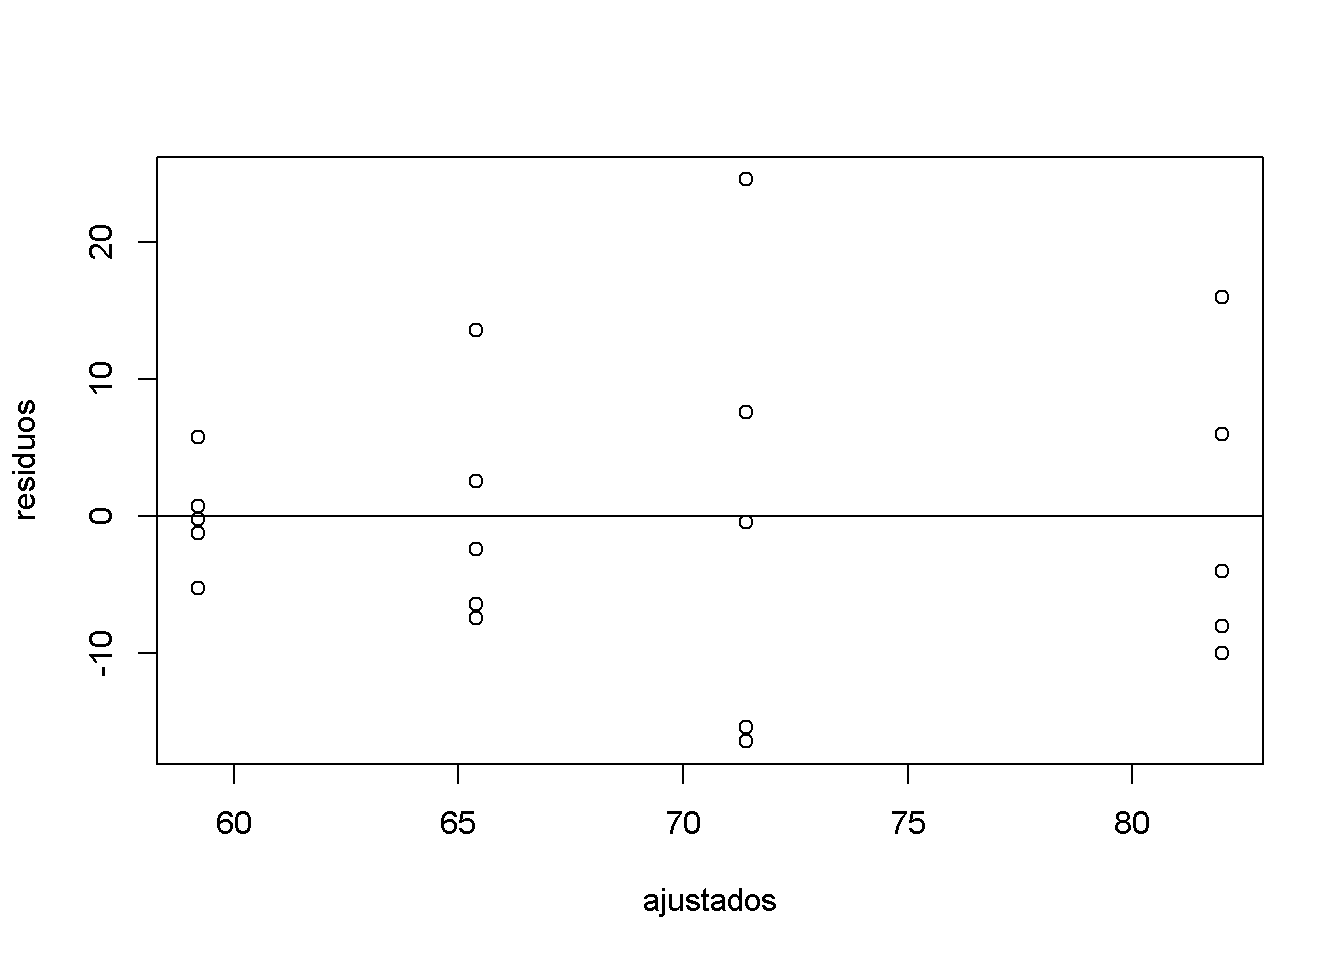
\includegraphics[width=0.6\linewidth]{02-Delinexp_files/figure-latex/unnamed-chunk-16-1} \end{center}

\hypertarget{analise-fatorial}{%
\chapter{Análise Fatorial}\label{analise-fatorial}}

A análise fatorial é um método estatístico utilizado para descrever a
variabilidade entre variáveis observadas e possivelmente correlacionadas
em termos de um número potencialmente menor de variáveis não observadas
chamadas fatores.

Assim, é possível que as variaçõess de três ou quatro variáveis
observadas possam ser explicadas por somente um fator, o que evidencia a
utilidade da análise fatorial para descrever um conjunto de dados
utilizando para isso apenas alguns fatores.

Diferentemente da análise de variância, regressão e análise
discriminante, onde uma das variáveis é identificada como a variável
dependente, examina-se todo o conjunto de relações interdependentes
entre variáveis.

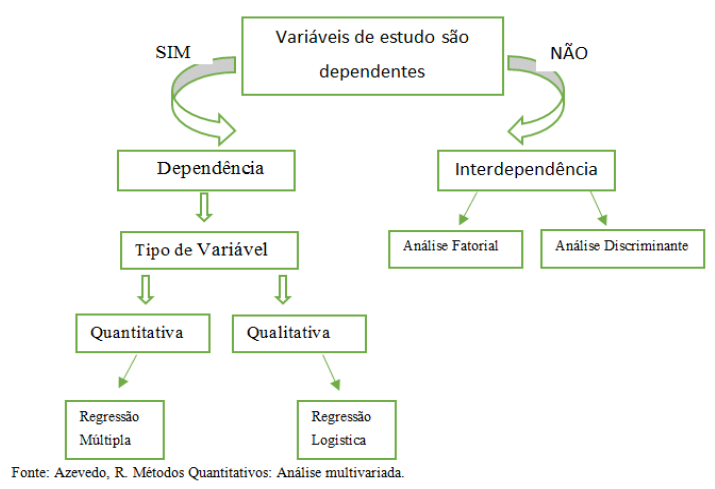
\includegraphics{anfat1.png}

A análise fatorial aborda o problema de analisar a estrutura das
inter-relações (correlações) entre um grande número de variáveis
(escores de testes, itens de testes, respostas de questionários),
definindo um conjunto de dimensões latentes comuns, chamados fatores.
Então, a análise fatorial, permite primeiro identificar as dimensões
separadas da estrutura e então determinar o grau em que cada variável é
explicada por cada dimensão. Uma vez que essas dimensões e a explicação
da cada variável estejam determinadas, os dois principais usos da
análise fatorial podem ser conseguidos:

\begin{itemize}
\item
  \textbf{Resumo}: ao resumir os dados, a análise fatorial obtém
  dimensões latentes que, quando interpretadas e compreendidas,
  descrevem os dados em um núumero muito menor de conceitos do que as
  variáveis individuais originais.
\item
  \textbf{Redução de dados}: pode ser obtida calculando escores para
  cada dimensão latente e substituindo as variáveis originais pelos
  mesmos.
\end{itemize}

As técnicas analíticas fatoriais podem ser classificadas quanto aos seus
objetivos como \textbf{exploratória} ou \textbf{confirmatória}.
Exploratória, útil na busca da estrutura em um conjunto de variáveis ou
como um método de redução de dados. Sob esta perspectiva, as técnicas
analíticas fatoriais ``consideram o que os dados oferecem''e não
estabelecem restriçoes \emph{a priori} sobre o número de componentes a
serem extraídos. O uso da análise fatorial em situações, que se deseja
testar hipóteses envolvendo questões sobre, quais variáveis deveriam ser
agrupadasem fator ou número exato de fatores, por exemplo, a análise
fatorial desempenha um papel confirmatório, ou seja, avalia o grau em
que os dados satisfazem a estrutura esperada.

Exemplo: em maketing, fatores associados às características do produto,
clientes e até mesmo da organização.

Em estudos visando analisar o inter-relacionamento e o agrupamento de
indivíduos, cidade ou regiões em grupos homogêneos em relação à
mobilidade, preferências pessoais, condições de desenvolvimento, entre
outras variáveis.

\hypertarget{pressupostos}{%
\section{Pressupostos}\label{pressupostos}}

A análise fatorial clássica exige que alguns pressupostos sejam
satisfeitos, quais sejam (MALHOTRA, 2001):

\begin{enumerate}
\def\labelenumi{\alph{enumi}.}
\item
  Normalidade dos dados: apesar deste pressuposto não ser crítico quando
  a estimação é realizada por mínimos quadrados ordinários, a exigência
  de normalidade auxilia na análise, evitando possíveis assimetrias e a
  presença de \emph{outliers}.
\item
  Variáveis quantitativas medidas em escala Intervalar ou de Razão. Esse
  pressuposto é crítico, pois a análise deve ser realizada com variáveis
  quantitatias e, frequentemente, alguns estudos são realizados
  utilizando variáveis ordinais (as quaiss são qualitativas) na análise
  fatorial clássica (o que é errado de muitas maneiras).
\item
  Como diretriz inicial deve haver ao menos quatro a cinco vezes mais
  observações do que variáveis.
\end{enumerate}

\hypertarget{estatisticas-associadas-a-analise-fatorial}{%
\section{Estatísticas Associadas a Análise
Fatorial}\label{estatisticas-associadas-a-analise-fatorial}}

Em geral, as estatísticas utilizadas no processo de análise fatorial são
(AAKER-KUMARDAY, 2001):

\begin{itemize}
\item
  Teste de esfericidade de Bartlett: estatística de teste usada para
  examinar a hipótese de que as variáveis não sejam correlacionadas na
  população, ou seja, a matriz de correlação da população é uma matriz
  identidade onde cada variável se correlaciona perfeitamente com ela
  própria (r=1), mas não apresenta correlação com as outras variáveis
  (r=0).
\item
  Matriz de correlação: o triângulo inferior da matriz exibe as
  correlações simples, r, entre todos os pares possíveis de variáveis
  incluídas na análise, enquanto os elementos da diagonal, que são todos
  iguais a 1, em geral são omitidos.
\item
  Comunalidade: porção da variância que uma variável compartilha com
  todas as outras variáveis consideradas, sendo também a proporção de
  variância explicada pelos fatores comuns.
\item
  Autovalor: representa a variância total explicada por cada fator.
\item
  Cargas fatoriais: correlação simples entre as variáveis e os fatores.
\item
  Gráfico das cargas dos fatores: gráfico das variáveis originais
  utilizando as cargas fatoriais como ordenadas.
\item
  Matriz de fatores ou matriz principal: contém as cargas fatoriais de
  todos as variáveis em todos os fatores extraídos.
\item
  Escores fatoriais: escores compostos estimados para cada entrevistado
  nos fatores derivados.
\item
  Medida de adequacidade da amostra de Kaiser-Meyer-Olkin (KMO): é o
  índice usado para avaliar a adequacidade da análise fatorial. Valores
  altos (entre 0,5 e 1,0) indicam que a análise fatorial é apropriada.
  Valores abaixo de 0,5 indicam que a análise fatorial pode ser
  inadequada.
\item
  Percentagem de variância: percentagem da variância total atribuída a
  cada fator.
\item
  Resíduos: diferenças entre as correlações observadas, dadas na matriz
  de correlação de entrada (input) e as correlações reproduzidas,
  conforme estimadas pela matriz de fatores.
\item
  Scree plot: gráfico dos autovalores versus número de fatores por ordem
  de extração.
\end{itemize}

Exemplo 1:

(MALHOTRA, 2001) Suponhamos que um pesquisador queira avaliar os
benefícios que os consumidores esperam de um dentifrício. Foi
entrevistada uma amostra de 30 pessoas em um supermercado, para que
indicassem seu grau de concordância com as seguintes afirmações,
utilizando uma escala de 7 pontos (1= discordância total, 7
=concordância total).

\begin{itemize}
\tightlist
\item
  V1: É importante comprar um creme dental que evite cáries.
\item
  V2: Gosto de um creme dental que clareie os dentes.
\item
  V3: Um creme dental deve fortificar as gengivas.
\item
  V4: Prefiro um creme dental que refresque o hálito.
\item
  V5: Manter os dentes sadios não é uma vantagem importante de um creme
  dental.
\item
  V6: O aspecto mais importante na compra de um creme dental é tornar os
  dentes atraentes.
\end{itemize}

Inicialmente podemos explorar algumas estatísticas descritivas
relacionadas às variáveis pesquisadas, utilizando a função
\texttt{summary}:

\begin{Shaded}
\begin{Highlighting}[]
\KeywordTok{require}\NormalTok{(readxl)}
\end{Highlighting}
\end{Shaded}

\begin{verbatim}
Carregando pacotes exigidos: readxl
\end{verbatim}

\begin{Shaded}
\begin{Highlighting}[]
\NormalTok{url <-}\StringTok{ "https://github.com/Smolski/softwarelivrer/raw/master/avancado/creme_dental_exemplo1.xlsx"}
\NormalTok{destfile <-}\StringTok{ "creme_dental_exemplo1.xlsx"}
\NormalTok{curl}\OperatorTok{::}\KeywordTok{curl_download}\NormalTok{(url, destfile)}
\NormalTok{creme_dental_exemplo1 <-}\StringTok{ }\KeywordTok{read_excel}\NormalTok{(destfile)}

\KeywordTok{attach}\NormalTok{(creme_dental_exemplo1)}
\KeywordTok{summary}\NormalTok{(creme_dental_exemplo1)}
\end{Highlighting}
\end{Shaded}

\begin{verbatim}
       v1             v2            v3            v4            v5     
 Min.   :1.00   Min.   :2.0   Min.   :1.0   Min.   :2.0   Min.   :1.0  
 1st Qu.:2.00   1st Qu.:3.0   1st Qu.:2.0   1st Qu.:3.0   1st Qu.:2.0  
 Median :4.00   Median :4.0   Median :4.0   Median :4.0   Median :3.5  
 Mean   :3.93   Mean   :3.9   Mean   :4.1   Mean   :4.1   Mean   :3.5  
 3rd Qu.:6.00   3rd Qu.:5.0   3rd Qu.:6.0   3rd Qu.:5.0   3rd Qu.:5.0  
 Max.   :7.00   Max.   :7.0   Max.   :7.0   Max.   :7.0   Max.   :7.0  
       v6      
 Min.   :2.00  
 1st Qu.:3.00  
 Median :4.00  
 Mean   :4.17  
 3rd Qu.:4.75  
 Max.   :7.00  
\end{verbatim}

\hypertarget{passos-da-analise-fatorial}{%
\section{Passos da Análise Fatorial}\label{passos-da-analise-fatorial}}

Basicamente, os seguintes passos conduzem a análise fatorial: entrada de
dados, cálculo das correlações entre as variáveis, extração inicial dos
fatores e a rotação da matriz.

\hypertarget{construcao-da-matriz-de-correlacao}{%
\subsection{Construção da Matriz de
Correlação}\label{construcao-da-matriz-de-correlacao}}

Entrada de Dados (BASE): os dados de entrada da análise fatorial
geralmente tomam a forma de um conjunto de valores de variáveis para
cada objeto ou indivíduo na amostra. Toda matriz, cujos componentes
ofereçam uma medida de similaridade entre variáveis, pode ser passível
de análise fatorial. A medida de similaridade não precisa ser uma
correlação, embora, geralmente, ou seja:

Para que a análise fatorial seja adequada, as variáveis devem ser
correlacionadas. Espera-se também que as variáveis altamente
correlacionadas umas com as outras se correlacionem também com o(s)
mesmo(s) fatore(s).

Note que existem correlações amostrais positivas e negativas
relativamente elevadas entre V1 (prevenção de cáries), V3 (gengivas
fortes) e V5 (dentes sadios). Espera-se que essas variáveis se
relacionem com o mesmo conjunto de fatores. Verificam-se também
correlações relativamente elevadas entre V2 (clareie os dentes), V4
(hálito puro) e V6 (dentes atraentes). Essas variáveis também devem
correlacionar-se com os mesmos fatores.

\begin{Shaded}
\begin{Highlighting}[]
\NormalTok{matcor <-}\StringTok{ }\KeywordTok{cor}\NormalTok{(creme_dental_exemplo1)}
\KeywordTok{print}\NormalTok{(matcor, }\DataTypeTok{digits =} \DecValTok{2}\NormalTok{)}
\end{Highlighting}
\end{Shaded}

\begin{verbatim}
        v1     v2     v3      v4      v5      v6
v1  1.0000 -0.053  0.873 -0.0862 -0.8576  0.0042
v2 -0.0532  1.000 -0.155  0.5722  0.0197  0.6405
v3  0.8731 -0.155  1.000 -0.2478 -0.7778 -0.0181
v4 -0.0862  0.572 -0.248  1.0000 -0.0066  0.6405
v5 -0.8576  0.020 -0.778 -0.0066  1.0000 -0.1364
v6  0.0042  0.640 -0.018  0.6405 -0.1364  1.0000
\end{verbatim}

\begin{Shaded}
\begin{Highlighting}[]
\KeywordTok{require}\NormalTok{(corrplot)}
\end{Highlighting}
\end{Shaded}

\begin{verbatim}
Carregando pacotes exigidos: corrplot
\end{verbatim}

\begin{verbatim}
corrplot 0.84 loaded
\end{verbatim}

\begin{Shaded}
\begin{Highlighting}[]
\KeywordTok{corrplot}\NormalTok{(matcor, }\DataTypeTok{method=}\StringTok{"circle"}\NormalTok{)}
\end{Highlighting}
\end{Shaded}

\begin{center}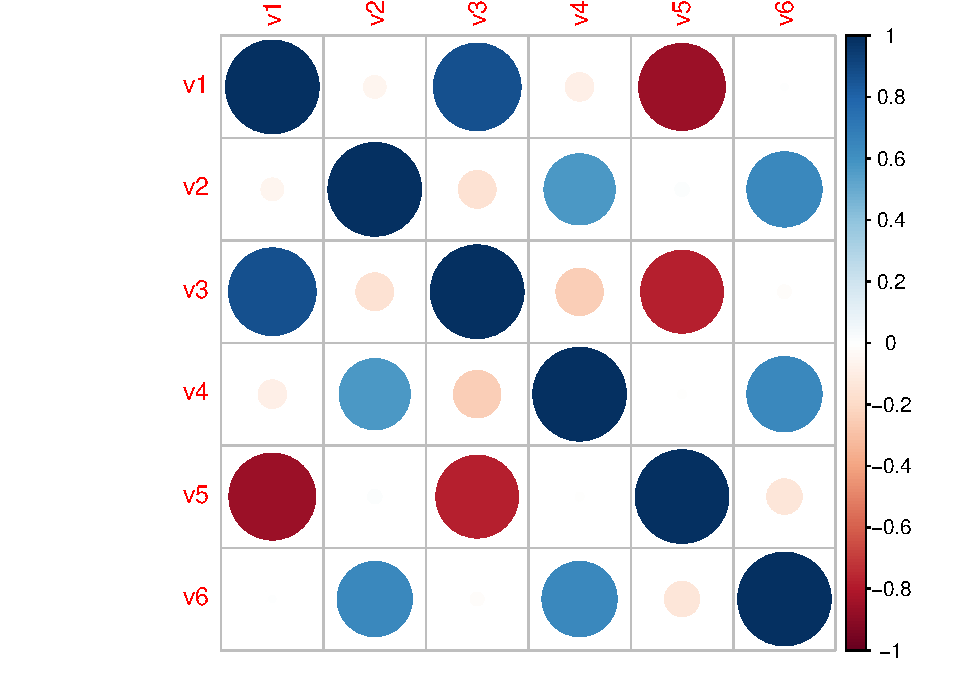
\includegraphics[width=0.6\linewidth]{03-AnaliseFat_files/figure-latex/unnamed-chunk-4-1} \end{center}

Na figura acima, as correlações estão em cor azul porque são positivas,
com tons mais fortes para as correlações mais altas.

Para testar a conveniência do modelo fatorial pode-se aplicar o teste de
esfericidade de Bartlett para testar a hipótese nula, de que as
variáveis não sejam correlacionadas na população. Um valor elevado da
estatística de teste favorece a rejeição da hipótese nula.

Também, a medida de adequacidade da amostra de Kaiser-Meyer-Olkin (KMO)
compara as magnitudes dos coeficientes de correlação observados com as
magnitudes dos coeficientes de correlação parcial. Pequenos valores de
KMO indicam que as correlações entre os pares de variáveis não podem ser
explicadas por outras variáveis, indicando que a análise fatorial não é
adequada.

Hipóteses:

Ho: A matriz de correlação da população é uma matriz identidade, ou seja
as variáveis não são correlacionadas na população.

H1: A matriz de correlação da população não é uma matriz identidade, ou
seja as variáveis são correlacionadas na população.

\begin{Shaded}
\begin{Highlighting}[]
\CommentTok{#install.packages("psych")}
\KeywordTok{require}\NormalTok{(psych)}
\end{Highlighting}
\end{Shaded}

\begin{verbatim}
Carregando pacotes exigidos: psych
\end{verbatim}

\begin{Shaded}
\begin{Highlighting}[]
\KeywordTok{cortest.bartlett}\NormalTok{(creme_dental_exemplo1)}
\end{Highlighting}
\end{Shaded}

\begin{verbatim}
R was not square, finding R from data
\end{verbatim}

\begin{verbatim}
$chisq
[1] 111.3

$p.value
[1] 9.017e-17

$df
[1] 15
\end{verbatim}

Veja que a hipótese nula de que a matriz de correlação da população seja
uma matriz identidade é rejeitada pelo teste de esfericidade de
Bartlett. A estatística qui-quadrado aproximada é 111,314, com 15 graus
de liberdade, significativa ao nível de 0,05.

\begin{Shaded}
\begin{Highlighting}[]
\KeywordTok{KMO}\NormalTok{(creme_dental_exemplo1)}
\end{Highlighting}
\end{Shaded}

\begin{verbatim}
Kaiser-Meyer-Olkin factor adequacy
Call: KMO(r = creme_dental_exemplo1)
Overall MSA =  0.66
MSA for each item = 
  v1   v2   v3   v4   v5   v6 
0.62 0.70 0.68 0.64 0.77 0.56 
\end{verbatim}

A estatística KMO maior que 0,5 também concorda quanto ao fato de que a
análise fatorial pode ser considerada uma técnica apropriada para
analisar a matriz de correlação.

\hypertarget{metodo-de-analise-fatorial}{%
\subsection{Método de Análise
Fatorial}\label{metodo-de-analise-fatorial}}

As duas abordagens básicas são a análise de componentes principais (ACP)
e a análise fatorial (AFC) comum ou análise fatorial exploratória (AFE),
embora existam diferentes métodos de extração de fatores da matriz de
correlações, que de forma geral, são métodos numericamente complexos. Na
análise de componentes principais, o objetivo da extração de fatores é
encontrar um conjunto de fatores que formem uma combinação linear das
variáveis originais ou da matriz de correlações. Assim, se as variáveis
X1 , X2 , X3 , \ldots{} , Xn são altamente correlacionadas entre si,
elas serão combinadas para formar um fator, e assim, sucessivamente, com
todas as demais variáveis da matriz de correlação.

A análise fatorial exploratória pode trazer informações importantes
sobre a estrutura multivariada de um instrumento de mensuração,
identificando os construtos teóricos.

O segundo objetivo da analise fatorial exploratória está relacionado à
redução de dados e descoberta de ponderações ótimas para as variáveis
mensuradas, de forma que um grande conjunto de variáveis possa ser
reduzido a um conjunto menor de índices sumários que tenham máxima
variabilidade e fidedignidade. A redução de dados é especialmente
possível pela aplicação da Análise dos Componentes Principais (ACP) e
não pelo uso da analise fatorial comum (AFC), havendo uma diferença
fundamental entre os dois métodos: a ACP trabalha com a variância total
observada, enquanto a AFC trabalha somente com a variância partilhada
dos itens (variância erro e variância única são excluídas) (LAROS,
2012).

Na AFC, os fatores são estimados para explicar as covariâncias entre as
variáveis observadas, portanto os fatores são considerados como as
causas das variáveis observadas. Já na ACP, os componentes são estimados
para representar a variância das variáveis observadas de uma maneira tão
econômica quanto possível. Os componentes principais são somas
otimamente ponderadas das variáveis observadas, neste sentido, as
variáveis observadas são consideradas as causas dos componentes
principais (LAROS, 2012).

Assim, recomenda-se a ACP, quando o objetivo é determinar o número
mínimo de fatores que respondem pela máxima variância nos dados, sendo
os fatores chamados componentes principais (MALHOTRA, 2001).

Obs.:

cor = TRUE: as componentes principais serão geradas a partir da matriz
de correlação.

cor = FALSE: as componentes principais serão geradas a partir da matriz
de covariância.

\begin{Shaded}
\begin{Highlighting}[]
\NormalTok{fit<-}\KeywordTok{princomp}\NormalTok{(creme_dental_exemplo1,}\DataTypeTok{cor=}\OtherTok{TRUE}\NormalTok{)}
\NormalTok{fit}
\end{Highlighting}
\end{Shaded}

\begin{verbatim}
Call:
princomp(x = creme_dental_exemplo1, cor = TRUE)

Standard deviations:
Comp.1 Comp.2 Comp.3 Comp.4 Comp.5 Comp.6 
1.6526 1.4893 0.6645 0.5842 0.4274 0.2919 

 6  variables and  30 observations.
\end{verbatim}

\begin{Shaded}
\begin{Highlighting}[]
\KeywordTok{summary}\NormalTok{(fit)}
\end{Highlighting}
\end{Shaded}

\begin{verbatim}
Importance of components:
                       Comp.1 Comp.2 Comp.3  Comp.4  Comp.5 Comp.6
Standard deviation     1.6526 1.4893 0.6645 0.58417 0.42735 0.2919
Proportion of Variance 0.4552 0.3697 0.0736 0.05688 0.03044 0.0142
Cumulative Proportion  0.4552 0.8249 0.8985 0.95536 0.98580 1.0000
\end{verbatim}

A função \texttt{summary(fit)} mostra a aplicação da análise de
componentes principais. O fator 1 responde por 45,52\% da variância
total. Da mesma forma, o segundo fator responde por 36,97\% da variância
total, sendo que os dois primeiros fatores respondem por 82,49\% da
variância total. Várias considerações devem integrar a análise do
núumero de fatores que devem ser usados na análise.

\hypertarget{determinacao-do-nuumero-de-fatores}{%
\subsection{Determinação do núumero de
fatores}\label{determinacao-do-nuumero-de-fatores}}

A fim de reduzir as informações presentes nas variáveis originais,
deve-se reduzir o número de fatores. Na literatura, diversos processos
são sugeridos: determinação a priori, observação dos autovalores,
representação gráfica (\textbf{scree plot}), testes de significância
entre outros.

\hypertarget{determinacao-a-priori}{%
\subsubsection{Determinação a priori}\label{determinacao-a-priori}}

Quando o pesquisador, com base na experiência que apresentação em
relação ao assunto, decide quantos fatores deseja utilizar.

\hypertarget{autovalores}{%
\subsubsection{Autovalores}\label{autovalores}}

Como o autovalor representa a quantidade de variância associada ao
fator, incluem-se apenas os fatores com variância maior que 1.

\hypertarget{grafico-de-declive-scree-plot}{%
\subsubsection{\texorpdfstring{Gráfico de declive (\textbf{scree
plot})}{Gráfico de declive (scree plot)}}\label{grafico-de-declive-scree-plot}}

Trata-se de uma representação gráfica dos autovalores associada ao
número de fatores na ordem de extração. O ponto em que a inclinação
suaviza indica o número de fatores a ser usados, que em geral é superior
ao revelado pelos autovalores.

\hypertarget{percentagem-da-variancia}{%
\subsubsection{Percentagem da
variância}\label{percentagem-da-variancia}}

Determina que o núumero de fatores extraídos seja de no mínimo 60\% da
variância.

\hypertarget{teste-de-significancia}{%
\subsubsection{Teste de significância}\label{teste-de-significancia}}

É possível reter apenas os fatores estatisticamente significativos com
base na significância estatística dos autovalores separados.

Abaixo vamos apresentar o \texttt{scree-plot}, em formato do gráfico de
barras para o nosso exemplo

\begin{Shaded}
\begin{Highlighting}[]
\KeywordTok{screeplot}\NormalTok{(fit)}
\end{Highlighting}
\end{Shaded}

\begin{center}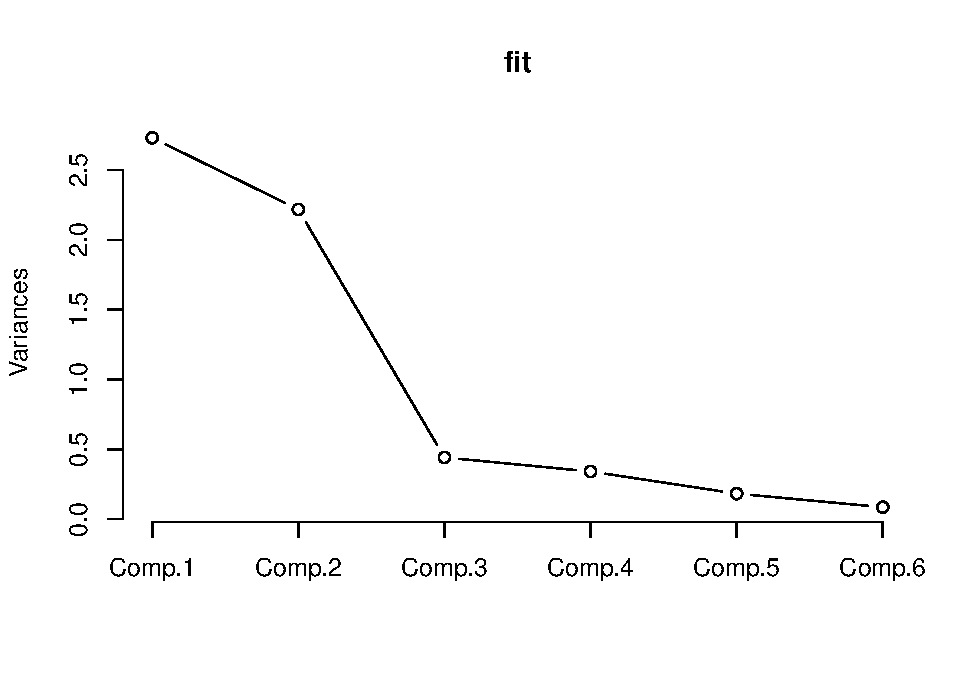
\includegraphics[width=0.6\linewidth]{03-AnaliseFat_files/figure-latex/unnamed-chunk-8-1} \end{center}

Note que as duas primeiras componentes, aparecem em destaque, ocorrendo
uma ligeira suavização das alturas nas demais colunas.

\begin{Shaded}
\begin{Highlighting}[]
\KeywordTok{plot}\NormalTok{(fit,}\DataTypeTok{type=}\StringTok{"lines"}\NormalTok{)}
\end{Highlighting}
\end{Shaded}

\begin{center}\includegraphics[width=0.6\linewidth]{03-AnaliseFat_files/figure-latex/unnamed-chunk-9-1} \end{center}

\hypertarget{analise-de-componentes-principais}{%
\subsection{Análise de Componentes
Principais}\label{analise-de-componentes-principais}}

Rodando a Análise de Componentes Principais no R, temos:

\begin{Shaded}
\begin{Highlighting}[]
\NormalTok{PCAdente<-}\KeywordTok{principal}\NormalTok{(creme_dental_exemplo1, }\DataTypeTok{nfactors=}\DecValTok{2}\NormalTok{,}
                \DataTypeTok{n.obs=}\DecValTok{30}\NormalTok{,}\DataTypeTok{rotate=}\StringTok{"none"}\NormalTok{, }\DataTypeTok{scores=}\OtherTok{TRUE}\NormalTok{)}
\NormalTok{PCAdente}
\end{Highlighting}
\end{Shaded}

\begin{verbatim}
Principal Components Analysis
Call: principal(r = creme_dental_exemplo1, nfactors = 2, rotate = "none", 
    n.obs = 30, scores = TRUE)
Standardized loadings (pattern matrix) based upon correlation matrix
     PC1   PC2   h2    u2 com
v1  0.93  0.25 0.93 0.074 1.1
v2 -0.30  0.80 0.72 0.277 1.3
v3  0.94  0.13 0.89 0.106 1.0
v4 -0.34  0.79 0.74 0.261 1.4
v5 -0.87 -0.35 0.88 0.122 1.3
v6 -0.18  0.87 0.79 0.210 1.1

                       PC1  PC2
SS loadings           2.73 2.22
Proportion Var        0.46 0.37
Cumulative Var        0.46 0.82
Proportion Explained  0.55 0.45
Cumulative Proportion 0.55 1.00

Mean item complexity =  1.2
Test of the hypothesis that 2 components are sufficient.

The root mean square of the residuals (RMSR) is  0.07 
 with the empirical chi square  3.94  with prob <  0.41 

Fit based upon off diagonal values = 0.98
\end{verbatim}

A matriz de fatores acima, resultante da análise de componentes
principais, é composta pelos coeficientes (cargas fatoriais) que
expressam as variáveis padronizadas em termos dos fatores. Valores altos
das cargas fatoriais, representam boa relação entre a variável e o
fator. Essa matriz não rotada, apresenta dificuldades para ser
interpretada pelo fato de que, em geral os fatores são correlacionados
com muitas variáveis.

Com o processo da rotação, a matriz de fatores resulta numa matriz mais
simples, sendo que a rotação não afeta as comunalidades e a porcentagem
da variância explicada. No entanto, a percentagem da variância explicada
por cada fator varia, sendo redistribuída por rotação (MALHOTRA, 2001).

Obs. comunalidades (\emph{communalities}) são quantidades das variâncias
(correlações) de cada variável explicada pelos fatores.

\hypertarget{matriz-rotada-do-fator}{%
\subsection{Matriz Rotada do Fator}\label{matriz-rotada-do-fator}}

Com o objetivo de possibilitar uma melhor interpretação dos fatores, é
prática comum fazer uma rotação ou uma transformação dos fatores.

O conjunto de cargas fatoriais, obtidas por qualquer método de solução
fatorial, quando o número de fatores comuns é maior do que um, não é
único, pois outros conjuntos equivalentes podem ser encontrados, por
transformações ortogonais de cargas.

Na rotação ortogonal, os eixos são mantidos em ângulo reto, sendo o
método mais utilizado o processo varimax. Esse método ortogonal de
rotação minimiza o número de variáveis com altas cargas sobre um fator
afim de permitir a interpretaçã dos fatores. A rotação ortogonal resulta
em fatores nãocorrelacionados ao passo que a rotação oblíqua não mantém
os eixos em ângulo reto e os fatores são correlacionados (MALHOTRA,
2001).

\begin{Shaded}
\begin{Highlighting}[]
\NormalTok{PCAdentevarimax<-}\KeywordTok{principal}\NormalTok{(creme_dental_exemplo1, }\DataTypeTok{nfactors=}\DecValTok{2}\NormalTok{,}
            \DataTypeTok{n.obs=}\DecValTok{30}\NormalTok{,}\DataTypeTok{rotate=}\StringTok{"varimax"}\NormalTok{,}\DataTypeTok{scores=}\OtherTok{TRUE}\NormalTok{)}
\NormalTok{PCAdentevarimax}
\end{Highlighting}
\end{Shaded}

\begin{verbatim}
Principal Components Analysis
Call: principal(r = creme_dental_exemplo1, nfactors = 2, rotate = "varimax", 
    n.obs = 30, scores = TRUE)
Standardized loadings (pattern matrix) based upon correlation matrix
     RC1   RC2   h2    u2 com
v1  0.96 -0.03 0.93 0.074 1.0
v2 -0.05  0.85 0.72 0.277 1.0
v3  0.93 -0.15 0.89 0.106 1.1
v4 -0.09  0.85 0.74 0.261 1.0
v5 -0.93 -0.08 0.88 0.122 1.0
v6  0.09  0.88 0.79 0.210 1.0

                       RC1  RC2
SS loadings           2.69 2.26
Proportion Var        0.45 0.38
Cumulative Var        0.45 0.82
Proportion Explained  0.54 0.46
Cumulative Proportion 0.54 1.00

Mean item complexity =  1
Test of the hypothesis that 2 components are sufficient.

The root mean square of the residuals (RMSR) is  0.07 
 with the empirical chi square  3.94  with prob <  0.41 

Fit based upon off diagonal values = 0.98
\end{verbatim}

Veja que na matriz rotada, o Fator 1 apresenta altos coeficientes para
as variáveis V1 (prevenção de cáries), V3 (gengivas fortes) e
coeficiente negativo para V5 (dentes sadios não é importante). O Fator 2
apresenta forte relação com V2 (clareie os dentes), V4 (hálito puro) e
V6 (dentes atraentes).

Rotulando:

Nesta fase é usual tentar dar nomes aos fatores. Em muitos casos, isto
requer um certo grau de imaginação:

\textbf{Fator 1}: Fator de benefício para a saúde.

\textbf{Fator 2}: Fator de benefício social.

Com os dois fatores acima, podemos concluir sobre o que o consumidor
espera de um creme dental.

\hypertarget{autovalores-1}{%
\subsection{Autovalores}\label{autovalores-1}}

Para acessar os eingenvalues (autovalores):

\begin{Shaded}
\begin{Highlighting}[]
\NormalTok{PCAdentevarimax}\OperatorTok{$}\NormalTok{values}
\end{Highlighting}
\end{Shaded}

\begin{verbatim}
[1] 2.73119 2.21812 0.44160 0.34126 0.18263 0.08521
\end{verbatim}

Confirmando, temos autovalores acima de 1, nos dois primeiros casos.

Para visualizar melhor a contribuição de cada variável (peso):

\begin{Shaded}
\begin{Highlighting}[]
\NormalTok{PCAdentevarimax}\OperatorTok{$}\NormalTok{loadings}
\end{Highlighting}
\end{Shaded}

\begin{verbatim}

Loadings:
   RC1    RC2   
v1  0.962       
v2         0.848
v3  0.933 -0.151
v4         0.855
v5 -0.934       
v6         0.885

                 RC1   RC2
SS loadings    2.687 2.263
Proportion Var 0.448 0.377
Cumulative Var 0.448 0.825
\end{verbatim}

Recurso importante na interpretação dos fatores, o gráfico das
variáveis, apresenta ao final do eixo, as variáveis que com cargas mais
altas sobre aquele fator. Quanto mais próximas da origem menores as
cargas destas variáveis sobre aquele fator. Variáveis distantes dos dois
eixos, estão relacionadas a ambos os fatores.

\begin{Shaded}
\begin{Highlighting}[]
\KeywordTok{biplot}\NormalTok{(PCAdentevarimax)}
\end{Highlighting}
\end{Shaded}

\begin{center}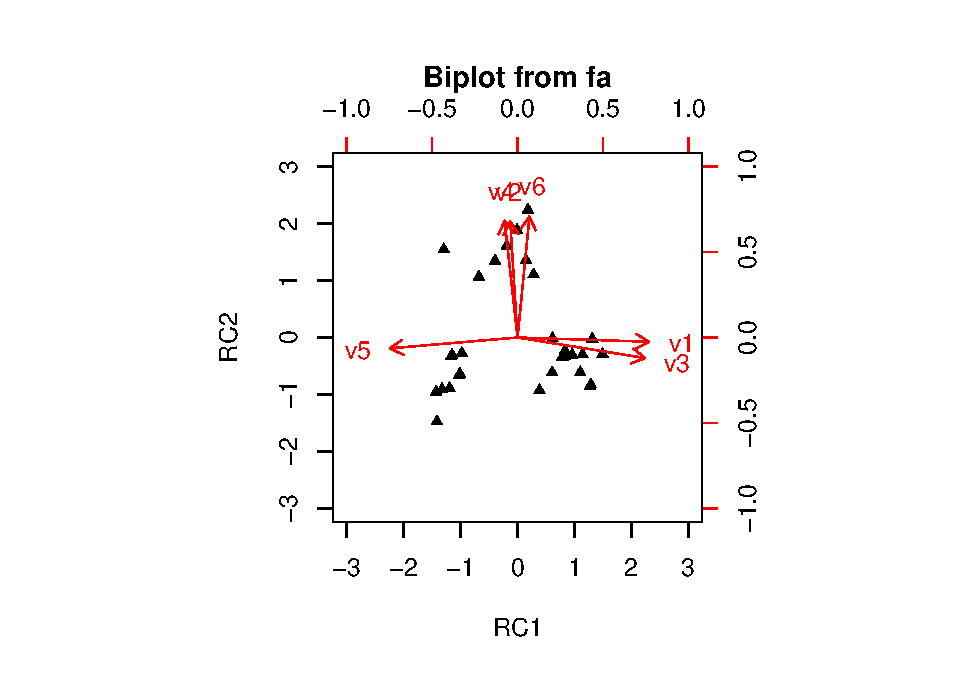
\includegraphics[width=0.6\linewidth]{03-AnaliseFat_files/figure-latex/unnamed-chunk-14-1} \end{center}

Os valores dos fatores obtidos para os 30 entrevistados encontram-se na
matriz de coeficiente de escore do componente mostrada abaixo. Esta
ajuda a entender como cada variável se relaciona aos escores dos
componentes calculados para cada participante. Para melhor compreensão
da análise dos escores dos entrevistados é importante especificar e
comentar o significado de cada fator:

\textbf{Fator 1}: Fator de benefício para a saúde.

\textbf{Fator 2}: Fator de benefício social.

Analisando os escores fatoriais dos entrevistados, destacamos a seguir
alguns entrevistados e seus respectivos resultados:

Entrevistado 18: 1.494934982

Este entrevistado se destacou como o primeiro colocado no ranqueamento,
obtendo o maior escore ponderado, demonstrando ser bastante atento à
prevenção de cáries, gengivas fortes e dentes sadios.

Entrevistado 29: 2.24121650

Este entrevistado se destacou em primeiro no segundo fator, apresentando
preocupação quanto ao beneffício social da dentição: boa aparência dos
dentes, hálito puro e boa aparência dos dentes.

Destacando-se os entrevistados de interesse, verifica-se:

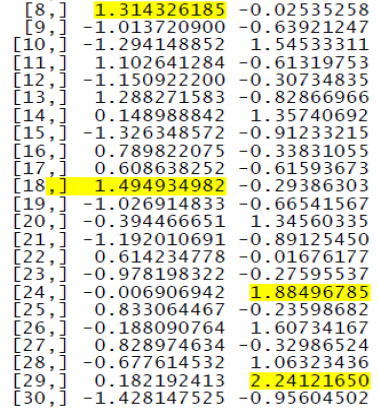
\includegraphics{anfat2.png}

\hypertarget{regressao-multipla}{%
\chapter{Regressão Múltipla}\label{regressao-multipla}}

\hypertarget{modelo-geral}{%
\section{Modelo geral}\label{modelo-geral}}

Um modelo de regressão múltipla é expresso como:

\[ 
y_{i} = \beta_0+\ \beta_1x_{1i}+\beta_2x_{2i}+\dots+\beta_kx_{ki}+\varepsilon_i\ 
\] \noindent em que:

\begin{itemize}
\item
  \(y_{i}\): valores da variável resposta, \(i = 1, 2,..., n\)
  observações;
\item
  \(x\): valores das variáveis explicativas, \(k = 1, 2,..., K\)
  variáveis;
\item
  \(\beta_k\): parâmetros do modelo;
\item
  \(\varepsilon_i\): erro aleatório.
\end{itemize}

A equação estimada para este modelo é definida como:

\[ 
y_{i} = b_0+\ b_1x_{1i}+b_2x_{2i}+\dots+b_kx_{ki} 
\] em que:

\begin{itemize}
\tightlist
\item
  \(b_k\): coeficientes estimados.
\end{itemize}

\hypertarget{variavel-dummy}{%
\section{Variável dummy}\label{variavel-dummy}}

Em algumas situações é necessário introduzir, como variável preditora
(independente), uma variável categórica no modelo de regressão linear
simples ou múltiplo, como por exemplo, local (urbano ou rural), área
(preservada ou degradada), etc, podendo ter mais que duas categorias.
Essa variável terá que ser codificada, utilizando somente códigos 0 e 1,
assim chamada variável dummy.

O número de variáveis dummy no modelo será sempre igual ao número de
categorias da variável preditora original menos 1. Por exemplo:

\begin{itemize}
\item
  Para a variável preditora ``local'' que assume valores - urbano ou
  rural, então têm-se a variável dummy local\_dummy assumindo 0 para
  rural e 1 para urbano; também, poderia ser utilizado 1 para rural e 0
  para urbano. Uma indicação é que a categoria que assume o valor 0 seja
  a categoria de referência.
\item
  Para a variável preditora ``grau de escolaridade''" que assume valores
  -- ensino fundamental, ensino médio, ensino superior, então têm-se as
  variáveis dummy: escola1 e escola2, assim definido:
\end{itemize}

\begin{enumerate}
\def\labelenumi{\alph{enumi}.}
\tightlist
\item
  escola1=0 e escola2=0 para ensino fundamental;
\item
  escola1=1 e escola2=0 para ensino médio;
\item
  escola1=0 e escola2=1 para ensino superior.
\end{enumerate}

\textbf{Exercício}:

\begin{enumerate}
\def\labelenumi{\arabic{enumi})}
\tightlist
\item
  Utilizando o banco de dados \texttt{ARVORE2}, ajuste um modelo de
  regressão linear simples para predizer a altura das árvores em função
  do diâmetro. Veja essa relação no diagrama de dispersão. Interprete os
  resultados.
\end{enumerate}

Relembrando Modelos de Regressão Linear Simples -- Curso Básico do
Software R:

\begin{itemize}
\tightlist
\item
  1.1 Ajustar a equação de regressão. Interpretá-la.
\item
  1.2 Encontrar e interpretar a significância da equação.
\item
  1.3 Encontrar e interpretar o coeficiente de determinação.
\item
  1.4 Analisar graficamente os resíduos.
\item
  1.5 Testar a normalidade dos resíduos.
\end{itemize}

Adicionalmente - Curso Avançado do Software R:

\begin{itemize}
\tightlist
\item
  1.6 Analisar pontos \emph{outliers} nos resíduos.
\end{itemize}

Para análise dos valores \emph{outliers} nos resíduos (\emph{residuals
standard} e \emph{residuals studentized}), utilizam-se os seguintes
comandos:

\texttt{rstudent(regressao)}

\texttt{rstandard(regressao)}

E o gráfico para verificar valores outliers nos resíduos:

\texttt{plot(rstudent(regressao))}

\texttt{plot(rstandard(regressao))}

Aqueles valores maiores que \textbar{}2\textbar{} são possíveis
outliers. Incluir uma linha y =2 e y=-2, para facilitar a visualização
de outliers.

\begin{itemize}
\tightlist
\item
  1.7 Analisar pontos influentes nos resíduos.
\end{itemize}

Para análise dos valores influentes, utiliza-se:

\texttt{dffits(regressao)}

Aqueles valores maiores que \texttt{2*(p/n)\^{}(1/2)} são possíveis
pontos influentes. Em que, p = número de parâmetros do modelo e n =
tamanho da amostra. O gráfico para detectar pontos influentes pode ser
elaborado pelo comando:

\texttt{plot(dffits(regressao))}

Aqueles valores maiores, em módulo, são possíveis influentes. Incluir
linhas para facilitar a visualização de pontos influentes.

Ainda, pode-se utilizar o comando \texttt{plot(regressao)} elabora
diferentes gráficos para o diagnóstico do modelo.

\begin{enumerate}
\def\labelenumi{\arabic{enumi})}
\setcounter{enumi}{1}
\item
  Ajuste um segundo modelo de regressão linear simples para predizer a
  altura das árvores em função da espécie. Veja essa relação no diagrama
  de dispersão. Interprete os resultados.
\item
  Ajuste um terceiro modelo de regressão múltipla para predizer a altura
  das árvores em função do diâmetro e da espécie. Interprete os
  resultados.
\end{enumerate}

\begin{Shaded}
\begin{Highlighting}[]
\KeywordTok{library}\NormalTok{(readxl)}
\NormalTok{url <-}\StringTok{ "https://github.com/Smolski/softwarelivrer/raw/master/avancado/arvore2.xlsx"}
\NormalTok{destfile <-}\StringTok{ "arvore2.xlsx"}
\NormalTok{curl}\OperatorTok{::}\KeywordTok{curl_download}\NormalTok{(url, destfile)}
\NormalTok{arvore2 <-}\StringTok{ }\KeywordTok{read_excel}\NormalTok{(destfile)}
\KeywordTok{attach}\NormalTok{(arvore2)}
\KeywordTok{head}\NormalTok{(arvore2)}
\end{Highlighting}
\end{Shaded}

\begin{verbatim}
# A tibble: 6 x 4
  Nomecientifico            diametro_cm altura_m especie
  <chr>                           <dbl>    <dbl>   <dbl>
1 Sebastiania commersoniana        52.2     15.2       0
2 Sebastiania commersoniana        95       17.3       0
3 Sebastiania commersoniana        67.3     16.3       0
4 Sebastiania commersoniana        46.3     14         0
5 Sebastiania commersoniana        64.1     15         0
6 Sebastiania commersoniana       122       22         0
\end{verbatim}

\begin{Shaded}
\begin{Highlighting}[]
\NormalTok{modelom=}\KeywordTok{lm}\NormalTok{(altura_m}\OperatorTok{~}\NormalTok{diametro_cm}\OperatorTok{+}\NormalTok{especie) }
\NormalTok{modelom}
\end{Highlighting}
\end{Shaded}

\begin{verbatim}

Call:
lm(formula = altura_m ~ diametro_cm + especie)

Coefficients:
(Intercept)  diametro_cm      especie  
    12.6959       0.0571      -1.6252  
\end{verbatim}

Modelo: \[
Y = 12,328 + 0,0576 x_1 – 1,423 x_2
\] Ou

\[
\text{Altura} = 12,328 + 0,0576\text{diâmetro} – 1,423\text{espécie}
\]

Verificando a significância de cada coeficiente do modelo de regressão
múltipla:

\begin{Shaded}
\begin{Highlighting}[]
\KeywordTok{summary}\NormalTok{(modelom)}
\end{Highlighting}
\end{Shaded}

\begin{verbatim}

Call:
lm(formula = altura_m ~ diametro_cm + especie)

Residuals:
   Min     1Q Median     3Q    Max 
-3.269 -0.766 -0.124  0.813  2.873 

Coefficients:
            Estimate Std. Error t value Pr(>|t|)    
(Intercept) 12.69592    0.38639   32.86  < 2e-16 ***
diametro_cm  0.05713    0.00445   12.84  < 2e-16 ***
especie     -1.62517    0.24459   -6.64  1.5e-09 ***
---
Signif. codes:  0 '***' 0.001 '**' 0.01 '*' 0.05 '.' 0.1 ' ' 1

Residual standard error: 1.19 on 102 degrees of freedom
Multiple R-squared:   0.7,  Adjusted R-squared:  0.694 
F-statistic:  119 on 2 and 102 DF,  p-value: <2e-16
\end{verbatim}

Verificar a significância do modelo completo.

Verificar o coeficiente de determinação do modelo.

Realizar análise dos resíduos.

\begin{itemize}
\tightlist
\item
  gráfico dos resíduos com cada variável preditora
\item
  resíduos padronizados para verificar outlier
\item
  verificar pontos infuentes
\end{itemize}

A interpretação dos termos de regressão é um pouco mais complicada. Em
geral, um modelo com múltiplos preditores indica a diferença média na
variável desfecho quando mudamos o valor de uma variável e mantemos a
outra constante.

Nesse caso, entre árvores de mesmo diâmetro (\(x_1\)), a diferença média
esperada da altura (y) para a espécie \emph{Syphoneugena reitzii} em
relação a espécie \emph{Sebastiania} commersoniana é de cerca de 1,42m a
menos (pois \(b_3\)=-1,42).

Da mesma forma, árvores da mesma espécie têm, em média, 0,05758m (pois
\(b_2\)=0,05758) a mais a cada 1 cm de diâmetro.

Como envolvem mais variáveis, não é possível resolver o modelo inteiro
num único gráfico. Como alternativa, pode-se plotar a reta para cada
espécie (variável categórica).

Primeiro, os pontos são plotados. O argumento
\texttt{type=\textquotesingle{}n\textquotesingle{}} indica que não é
para acrescentar nenhum ponto ao gráfico. Em seguida, os pontos são
acrescentados separadamente, com a função points, a qual acrescenta
pontos ao gráfico, sendo que o colchetes \texttt{{[}espécie==0{]}}
seleciona somente os casos desejados.

Por fim, acrescentamos as retas de regressão para cada resposta a
variável independente espécie. Usamos a função \texttt{coef} para
extrair os coeficientes de interesse.

\begin{Shaded}
\begin{Highlighting}[]
\KeywordTok{plot}\NormalTok{(diametro_cm,altura_m)}
\CommentTok{# Gera o gráfico sem pontos}
\KeywordTok{plot}\NormalTok{(diametro_cm,altura_m,}\DataTypeTok{type=}\StringTok{'n'}\NormalTok{) }
\CommentTok{# Acrescenta os pontos}
\KeywordTok{points}\NormalTok{(diametro_cm[especie}\OperatorTok{==}\DecValTok{0}\NormalTok{],altura_m[especie}\OperatorTok{==}\DecValTok{0}\NormalTok{],}\DataTypeTok{col=}\StringTok{'blue'}\NormalTok{)}
\KeywordTok{points}\NormalTok{(diametro_cm[especie}\OperatorTok{==}\DecValTok{1}\NormalTok{],altura_m[especie}\OperatorTok{==}\DecValTok{1}\NormalTok{],}\DataTypeTok{col=}\StringTok{'red'}\NormalTok{)}
\CommentTok{# Acrescenta as linhas}
\KeywordTok{abline}\NormalTok{(}\KeywordTok{coef}\NormalTok{(modelom)[}\DecValTok{1}\NormalTok{], }\KeywordTok{coef}\NormalTok{(modelom)[}\DecValTok{2}\NormalTok{], }\DataTypeTok{col=}\StringTok{'blue'}\NormalTok{)}
\KeywordTok{abline}\NormalTok{(}\KeywordTok{coef}\NormalTok{(modelom)[}\DecValTok{1}\NormalTok{]}\OperatorTok{+}\KeywordTok{coef}\NormalTok{(modelom)[}\DecValTok{3}\NormalTok{], }\KeywordTok{coef}\NormalTok{(modelom)[}\DecValTok{2}\NormalTok{], }\DataTypeTok{col=}\StringTok{'red'}\NormalTok{)}
\end{Highlighting}
\end{Shaded}

\begin{center}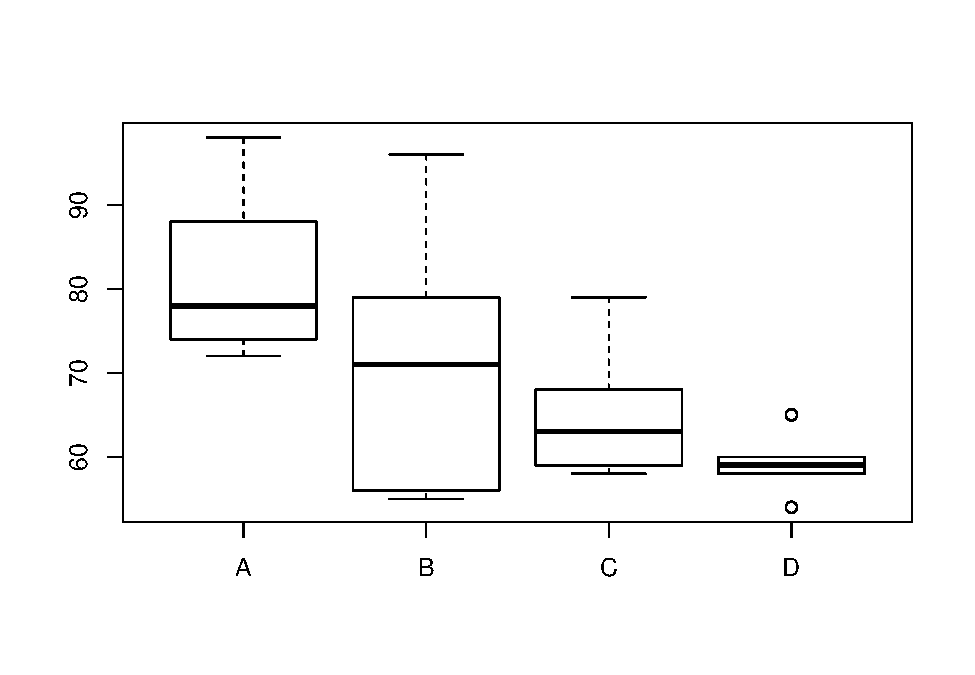
\includegraphics[width=0.6\linewidth]{04-RegMult_files/figure-latex/unnamed-chunk-5-1} \end{center}

\hypertarget{metodos-selecao-de-variaveis-na-regressao-multipla}{%
\section{Métodos seleção de variáveis na regressão
múltipla}\label{metodos-selecao-de-variaveis-na-regressao-multipla}}

\hypertarget{full-model-modelo-completo}{%
\subsection{Full model -- Modelo
completo}\label{full-model-modelo-completo}}

Sintaxe no software R para um modelo de regressão múltipla com três
variáveis preditivas:

\texttt{regressao=lm(y\textasciitilde{}x1+x2+x3)}

\texttt{summary(regressao)}

Existem três métodos de seleção de variáveis para modelos de regressão
múltipla: \emph{backward}, \emph{forward} e \emph{stepwise}.

\texttt{regressao=step(lm(y\textasciitilde{}x1+x2+x3),direction\ =\ \textquotesingle{}método\textquotesingle{})}

\hypertarget{procedimento-backward}{%
\subsection{Procedimento backward}\label{procedimento-backward}}

Considera todas as variáveis inicialmente, testando posteriormente, a
permanência de cada uma no modelo. Se p \(\leq\) 15\%, permanece no
modelo (saiu do modelo não entra mais) (Riboldi, 2005).

Passo 1) Ajustar o modelo completo de m variáveis e obter
\(SQR^{c}_{eg}\) e \(\sigma^{2}\);

Passo 2) Para cada uma das m variáveis do modelo completo do passo 1,
considerar o modelo reduzido -- retirando esta variável -- e calcular
\(SQR^{r}_{eg}\) para obter o valor da estatística (slide 24);

Passo 3) Achar o mínimo dos m valores da estatística obtidos no passo 2,
denotado por F\textsubscript{min};

Passo 4) Seja F\textsubscript{out} o valor da distribuição F com 1 e
(n-m-1) gl;

\begin{itemize}
\item
  Se F\textsubscript{min} \textgreater{} F\textsubscript{out}:
  interromper o processo e optar pelo modelo completo desta etapa;
\item
  Se F\textsubscript{min} \textless{} F\textsubscript{out}: voltar ao
  passo 1, iniciando nova etapa em que o modelo completo tem (m-1)
  variáveis -- dada a eliminação da variável cuja estatística é igual a
  F\textsubscript{min}.
\end{itemize}

\hypertarget{procedimento-forward}{%
\subsection{Procedimento forward}\label{procedimento-forward}}

Inclui uma variável de cada vez, se p \(\leq\) 20\%, entra no modelo.
Este método não testa a permanência da variável (entrou no modelo não
sai mais) (Riboldi, 2005).

Passo 1) Ajustar o modelo reduzido de m variáveis e obter
\(SQR^{c}_{eg}\);

Passo 2) Para cada variável não pertencente ao modelo do passo 1,
considerar o modelo completo com adição desta variável extra e calcular
\(SQR^{r}_{eg}\) e \(\sigma^{2}\) para obter o valor da estatística
(slide 26);

Passo 3) Achar o máximo dos valores da estatística obtidos no passo 2,
denotado por F\textsubscript{max};

Passo 4) Seja F\textsubscript{in} o valor da distribuição F com 1 e
(n-m) gl;

\begin{itemize}
\item
  Se F\textsubscript{max} \textgreater{} F\textsubscript{in}: voltar ao
  passo 1, iniciando nova etapa em que o modelo reduzido tem (m+1)
  variáveis -- dada a inclusão da variável cuja estatística é igual a
  F\textsubscript{max}.
\item
  Se F\textsubscript{max} \textless{} F\textsubscript{in}: interromper o
  processo e optar pelo modelo reduzido desta etapa;
\end{itemize}

\hypertarget{procedimento-stepwise}{%
\subsection{Procedimento stepwise}\label{procedimento-stepwise}}

Inclui as variáveis passo-a-passo e testa a permanência (as variáveis
podem entrar e sair do modelo) (Riboldi, 2005).

Passo 1) Ajustar o modelo reduzido de m variáveis e obter
\(SQR^{r}_{eg}\);

Passo 2) Para cada variável não pertencente ao modelo do passo 1,
considerar o modelo completo - com adição desta variável extra - e
calcular \(SQR^{c}_{eg}\) e \(\sigma^{2}\) para obter o valor da
estatística (slide 26);

Passo 3) Achar o máximo dos valores da estatística obtidos no passo 2,
denotado por F\textsubscript{max};

Passo 4) Seja Fin o valor da distribuição F com 1 e (n-m) gl;

\begin{itemize}
\item
  Se Fmax \textgreater{} Fin -\textgreater{} passar ao passo 5, com
  modelo completo composto por (m+1) variáveis -- as m variáveis do
  modelo do passo 1 e a variável cuja estatística é igual a Fmax.
\item
  Se Fmax \textless{} Fin -\textgreater{} passar ao passo 5, com modelo
  completo igual ao modelo do passo 1 ou encerrar o processo se no passo
  8 da etapa anterior, nenhuma variável tiver sido eliminada;
\end{itemize}

Passo 5) Ajustar o modelo completo de k variáveis -- sendo k igual a m
ou (m+1), e obter \(SQR^{c}_{eg}\) e \(\sigma^{2}\);

Passo 6) Para cada uma das k variáveis do modelo completo do passo 5,
considerar o modelo reduzido -- retirando esta variável -- e calcular
\(SQR^{r}_{eg}\) para obter o valor da estatística;

Passo 7) Achar o mínimo dos k valores da estatística obtidos no passo 6,
denotado por F\textsubscript{min};

Passo 8) Seja F\textsubscript{out} o valor da distribuição F com 1 e
(n-k-1) gl;

\begin{itemize}
\item
  Se F\textsubscript{min} \textgreater{} F\textsubscript{out}: não
  eliminar nenhuma variável e voltar ao passo 1, iniciando nova etapa
  com modelo reduzido com k variáveis ou encerrar o processo de no passo
  4 nenhuma variável tiver sido anexada;
\item
  Se Fmin \textless{} Fout: eliminar a variável cuja estatística é igual
  a Fmin e voltar ao passo 1 iniciando nova etapa com modelo reduzido
  com (k-1) variáveis.
\end{itemize}

\begin{figure}
\centering
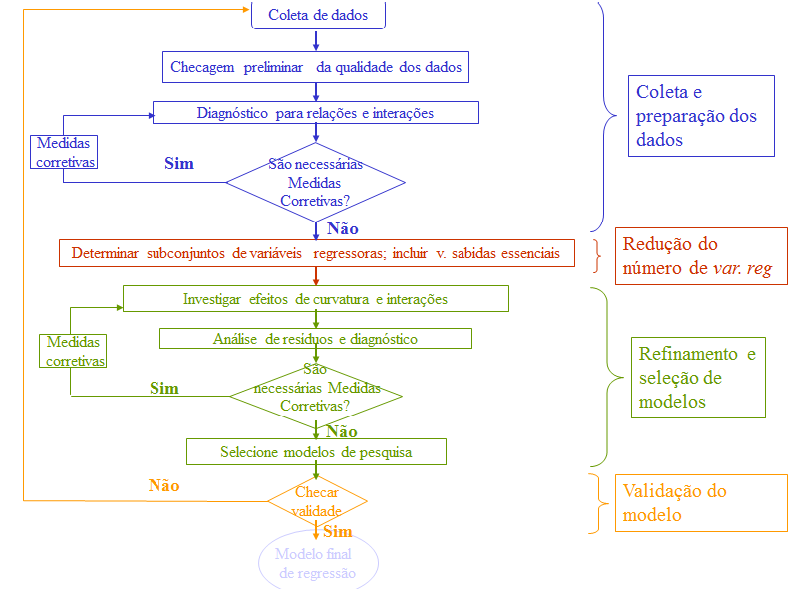
\includegraphics{regress1.png}
\caption{Modelagem estatística}
\end{figure}

\hypertarget{regressao-logistica}{%
\chapter{Regressão Logística}\label{regressao-logistica}}

A técnica de regressão logística é uma ferramenta estatística utilizada
nas análises preditivas. O interesse em mensurar a probabilidade de um
evento ocorrer é extremamente relevante em diversas áreas, como por
exemplo em Marketing, Propaganda e Internet, na Aplicação da Lei e
Detecção de Fraude, na Assistência Médica, com relação aos Riscos
Financeiros e Seguros ou mesmo estudando a Força de Trabalho. É
imprescindível elevar o conhecimento sobre quais clientes possuem maior
propensão à responder o contato de marketing, quais transações serão
fraudulentas, quais e-mails são \emph{spam}, quem efetivamente fará o
pagamento de uma obrigação ou mesmo qual criminoso reincidirá.\footnote{Para
  mais exemplos como estes sobre análises preditivas, ver SIEGEL
  (\protect\hyperlink{ref-Siegel2017}{2017}).}

\hypertarget{o-modelo}{%
\section{O modelo}\label{o-modelo}}

O modelo de regressão logística é utilizado quando a variável dependente
é binária, categórica ordenada ou mesmo categórica desordenada (quando
não há relação hierárquica entre elas). Abaixo exemplificam-se algumas
perguntas que podem levar a estes três tipos de variáveis.

\begin{longtable}[]{@{}lll@{}}
\caption{\label{tab:logtip}Tipos de variáveis}\tabularnewline
\toprule
\endhead
\begin{minipage}[t]{0.30\columnwidth}\raggedright
\textbf{Variável dependente binária:}\strut
\end{minipage} & \begin{minipage}[t]{0.30\columnwidth}\raggedright
Você votou na última eleição?\strut
\end{minipage} & \begin{minipage}[t]{0.30\columnwidth}\raggedright
0 - Não; 1 - Sim\strut
\end{minipage}\tabularnewline
\begin{minipage}[t]{0.30\columnwidth}\raggedright
\textbf{Variável dependente categórica ordenada:}\strut
\end{minipage} & \begin{minipage}[t]{0.30\columnwidth}\raggedright
Você concorda ou desconcorda com o presidente?\strut
\end{minipage} & \begin{minipage}[t]{0.30\columnwidth}\raggedright
1 - Disconcordo; 2 - Neutro; 3 - Concordo\strut
\end{minipage}\tabularnewline
\begin{minipage}[t]{0.30\columnwidth}\raggedright
\textbf{Variável dependente categórica não ordenada:}\strut
\end{minipage} & \begin{minipage}[t]{0.30\columnwidth}\raggedright
Se as eleições fossem hoje, em que partido você votaria?\strut
\end{minipage} & \begin{minipage}[t]{0.30\columnwidth}\raggedright
1 - Democratas; 2 - Qualquer um; 3 - Republicanos\strut
\end{minipage}\tabularnewline
\bottomrule
\end{longtable}

Fonte: Adaptado de TORRES-REYNA
(\protect\hyperlink{ref-Torres-Reyna2014}{2014}).

Nota-se primeiramente que em sendo somente a variável dependente
\textbf{binária} (0 e 1), é detectada a presença ou não de determinada
característica da variável a ser estudada pelo pesquisador. Outros
exemplos abrangem a qualificação dos indivíduos estaudados em sendo do
sexo feminino (1) ou do sexo masculino (0), se a empresa analisada está
inadimplente (1) ou não (0) no mês de referência, etc. Por outro lado,
quando a variável dependente é \textbf{categórica ordenada}, há uma
hierarquia determinada entre as variáveis resposta (neste caso entre
Disconcordo, Neutro e Concordo). No terceiro exemplo, a variável
resposta é \textbf{categórica não ordenada} não possuindo nenhuma
relação de ordem entre elas (Democratas, Qualquer um, Republicanos).

A regressão logística a ser estudada neste capítulo será com a variável
resposta dependente binária, portanto, tratando os grupos de interesse
(variável dependente) com valores de 0 e 1. Sua funcionalidade se ocupa
de prever a probabilidade de uma observação estar no grupo igual a 1
(``eventos''), em relação ao grupo igual a zero (``não eventos'').

Para a estimação dos coeficientes das variáveis independentes, são
utilizados o valor logit ou a razão de desigualdades (HAIR et al.,
\protect\hyperlink{ref-Hair2009}{2009}):

\[
Logit_i=ln\left (\frac{prob_{eventos}}{1-prob_{eventos}}  \right )=b_0+b_1X_1+\ldots+b_nX_n
\]

ou

\[
Logit_i=\left (\frac{prob_{eventos}}{1-prob_{eventos}}  \right )=e^{b_0+b_1X_1+\ldots+b_nX_n}
\]

Algumas características importantes da regressão logística: a análise é
semelhante à regressão linear simples/múltipla (possui a relação entre a
variável dependente e a(s) variável(is) independente(s)); possui testes
estatísticos diretos, incorporando variáveis métricas e não-métricas,
com efeitos não-lineares; é menos afetada pela não satisfação de
normalidade dos dados (pois o termo de erro da variável discreta segue a
distribuição binomial) e; foi elaborada para que seja prevista a
probabilidade de determinado evento ocorrer (HAIR et al.,
\protect\hyperlink{ref-Hair2009}{2009}).

Para otimizar o tempo do estudante, é recomendada a instalação prévia
dos pacotes no RStudio a serem utilizados neste capítulo. Segue abaixo o
comando a ser efetuado no console do RStudio:

\texttt{install.packages(c("readr","mfx","caret","pRoc",}
\texttt{"ResourceSelection","modEvA","foreign","stargazer"))}

\hypertarget{regressao-logistica-simples}{%
\section{Regressão Logística
Simples}\label{regressao-logistica-simples}}

Este primeiro exemplo tratará da regressão logística simples, portanto,
utilizando somente uma variável independente, neste caso numérica. Os
dados são originados do livro de HOSMER; LEMESCHOW
(\protect\hyperlink{ref-Hosmer2000}{2000}), tratando-se de uma amostra
com 100 pessoas. A variável dependente é a ocorrência ou não (1 ou 0) de
doença coronária cardíaca (CHD), associando-se com a idade (AGE) dos
indivíduos, criando assim um modelo de regressão logística.

\begin{Shaded}
\begin{Highlighting}[]
\KeywordTok{require}\NormalTok{(readr)}
\end{Highlighting}
\end{Shaded}

\begin{verbatim}
Carregando pacotes exigidos: readr
\end{verbatim}

\begin{Shaded}
\begin{Highlighting}[]
\NormalTok{chd <-}\StringTok{ }\KeywordTok{read_delim}\NormalTok{(}\StringTok{"https://goo.gl/uDAAHv"}\NormalTok{, }
    \StringTok{";"}\NormalTok{, }\DataTypeTok{escape_double =} \OtherTok{FALSE}\NormalTok{, }\DataTypeTok{col_types =} \KeywordTok{cols}\NormalTok{(}\DataTypeTok{CHD =} \KeywordTok{col_factor}\NormalTok{(}\DataTypeTok{levels =} \KeywordTok{c}\NormalTok{())), }
    \DataTypeTok{trim_ws =} \OtherTok{TRUE}\NormalTok{)}

\KeywordTok{summary}\NormalTok{(chd)}
\end{Highlighting}
\end{Shaded}

\begin{verbatim}
      AGE            AGRP      CHD   
 Min.   :20.0   Min.   :1.00   0:57  
 1st Qu.:34.8   1st Qu.:2.75   1:43  
 Median :44.0   Median :4.00         
 Mean   :44.4   Mean   :4.48         
 3rd Qu.:55.0   3rd Qu.:7.00         
 Max.   :69.0   Max.   :8.00         
\end{verbatim}

Observa-se na figura abaixo a dispersão dos ``eventos'' e dos
``nao-eventos'' da CHD relacionando-se com a variável idade (AGE).

\begin{Shaded}
\begin{Highlighting}[]
\KeywordTok{require}\NormalTok{(ggplot2)}

\KeywordTok{ggplot}\NormalTok{(chd, }\KeywordTok{aes}\NormalTok{(}\DataTypeTok{x=}\NormalTok{AGE, }\DataTypeTok{y=}\NormalTok{CHD)) }\OperatorTok{+}\StringTok{ }
\StringTok{  }\KeywordTok{geom_point}\NormalTok{() }\OperatorTok{+}\StringTok{ }
\StringTok{  }\KeywordTok{stat_smooth}\NormalTok{(}\DataTypeTok{method=}\StringTok{"glm"}\NormalTok{, }\DataTypeTok{method.args=}\KeywordTok{list}\NormalTok{(}\DataTypeTok{family=}\StringTok{"binomial"}\NormalTok{), }\DataTypeTok{se=}\OtherTok{FALSE}\NormalTok{)}
\end{Highlighting}
\end{Shaded}

\begin{figure}[h]

{\centering 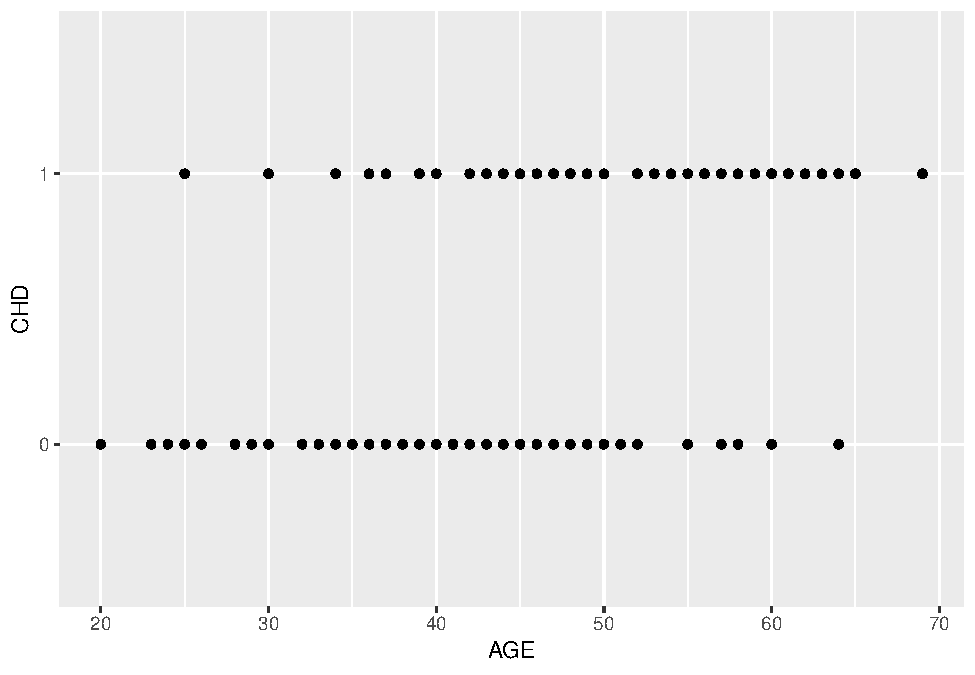
\includegraphics[width=0.6\linewidth]{05-RegLogist_files/figure-latex/dispev-1} 

}

\caption{Dispersão de evendos e não-eventos}\label{fig:dispev}
\end{figure}

Monta-se então o modelo de regressão logística com a variável dependente
CHD e a variável independente AGE. Abaixo é demonstrada a descrição da
equação utilizando o comando \texttt{summary()} para o modelo m1 com a
sintaxe básica:

\texttt{glm(Y\textasciitilde{}modelo,\ family=binomial(link="logit"))}

Assim é obtida a função de ligação estimada do modelo:

\[
\hat g(CHD) = -5,309 +0,1109AGE
\]

\begin{Shaded}
\begin{Highlighting}[]
\NormalTok{m1=}\KeywordTok{glm}\NormalTok{(CHD}\OperatorTok{~}\NormalTok{AGE, }\DataTypeTok{family =} \KeywordTok{binomial}\NormalTok{(}\DataTypeTok{link=}\StringTok{"logit"}\NormalTok{), }\DataTypeTok{data =}\NormalTok{ chd)}
\KeywordTok{summary}\NormalTok{(m1)}
\end{Highlighting}
\end{Shaded}

\begin{verbatim}

Call:
glm(formula = CHD ~ AGE, family = binomial(link = "logit"), data = chd)

Deviance Residuals: 
   Min      1Q  Median      3Q     Max  
-1.972  -0.846  -0.458   0.825   2.286  

Coefficients:
            Estimate Std. Error z value Pr(>|z|)    
(Intercept)  -5.3095     1.1337   -4.68  2.8e-06 ***
AGE           0.1109     0.0241    4.61  4.0e-06 ***
---
Signif. codes:  0 '***' 0.001 '**' 0.01 '*' 0.05 '.' 0.1 ' ' 1

(Dispersion parameter for binomial family taken to be 1)

    Null deviance: 136.66  on 99  degrees of freedom
Residual deviance: 107.35  on 98  degrees of freedom
AIC: 111.4

Number of Fisher Scoring iterations: 4
\end{verbatim}

Se observa o intercepto com o valor de -5,309, sendo que para a análise
aqui proposta da relação entre CHD e AGE não obtém-se um significado
prático para este resultado. No entanto, a variável de interesse é
idade, que no modelo de regressão obteve o coeficiente de 0,1109. Pelo
fato de ser positivo informa que quando a idade (AGE) se eleva,
elevam-se as chances de ocorrência de CHD. De igual forma, nota-se que
há significância estatística a \(p=0,001\) na utilização da variável AGE
para o modelo, mostrando que possui importância ao modelo de regressão
proposto.

Por fim, o modelo é utilizado para construção da predição de todos os
valores das idades de todos os indivíduos desta amostra. Para isto, será
criada um novo objeto contendo somente a variável dependente do modelo
(AGE) e em sequida, é criada nova coluna constando os valores preditos.
Assim, pode ser plotado um gráfico completo com todas as probabilidades
desta base de dados:

\begin{Shaded}
\begin{Highlighting}[]
\CommentTok{# Filtrando a idade dos indivíduos}
\NormalTok{IDADE<-chd[,}\DecValTok{1}\NormalTok{]  }

\CommentTok{# Criando campo de predição para cada idade dos indivíduos }
\NormalTok{IDADE}\OperatorTok{$}\NormalTok{PRED=}\KeywordTok{predict}\NormalTok{(m1, }\DataTypeTok{newdata=}\NormalTok{IDADE, }\DataTypeTok{type=}\StringTok{"response"}\NormalTok{)}

\CommentTok{# Plotando a probabilidade predita pelo modelo}
\KeywordTok{require}\NormalTok{(ggplot2)}
\KeywordTok{ggplot}\NormalTok{(IDADE, }\KeywordTok{aes}\NormalTok{(}\DataTypeTok{x=}\NormalTok{AGE, }\DataTypeTok{y=}\NormalTok{PRED)) }\OperatorTok{+}\StringTok{ }
\StringTok{  }\KeywordTok{geom_point}\NormalTok{()}
\end{Highlighting}
\end{Shaded}

\begin{figure}[h]

{\centering 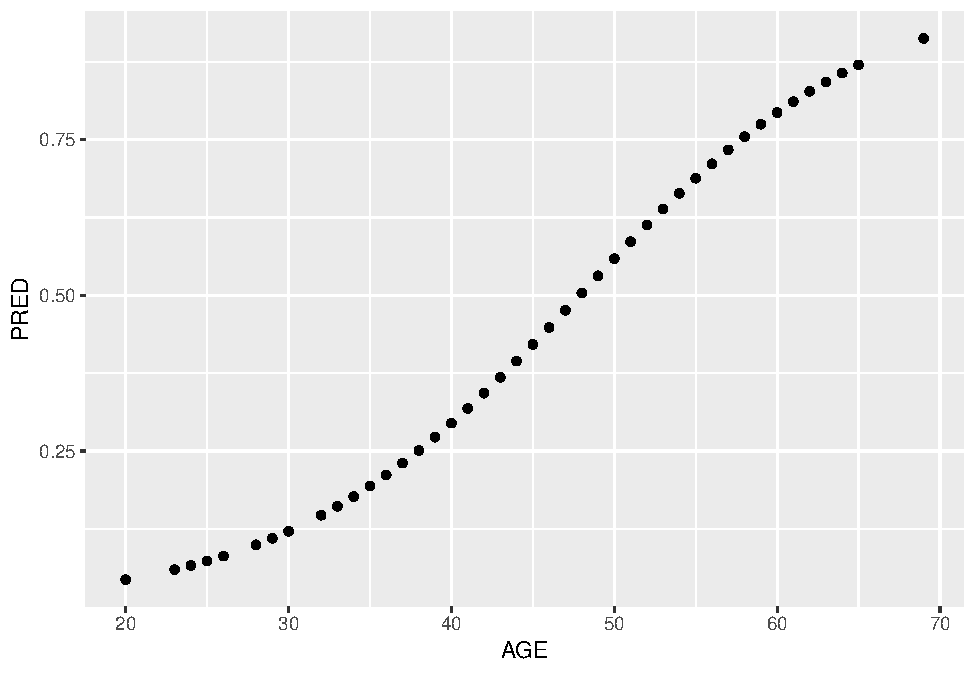
\includegraphics[width=0.6\linewidth]{05-RegLogist_files/figure-latex/distrpred-1} 

}

\caption{Distribuição das probabilidades preditas}\label{fig:distrpred}
\end{figure}

\hypertarget{estimando-a-razao-de-chances}{%
\subsection{Estimando a Razão de
Chances}\label{estimando-a-razao-de-chances}}

O modelo de regressão logística, porém, traz os resultados dos
estimadores na forma logarítma, ou seja, o log das chances da variável
idade no modelo é 0,1109. No entanto, para uma interpretação mais
enriquecida da relação da idade com o CHD é necessária a transformação
deste coeficiente, ou seja, que seja efetuada a exponenciação da(s)
variavel(eis) da regressão. Assim, obtém-se a razão das chances (OR -
Odds Ratio em inglês) para as variáveis independentes.

Uma maneira prática de se obter a razão de chances no RStudio é
utilizando o pacote \(mfx\). Novamente o intercepto não nos interessa
nesta análise mas sim a variável AGE. Como demonstrado abaixo, o
resultado da razão de chances da variável AGE foi de 1,1173, o que pode
assim ser interpretado: para cada variação unitária na idade (AGE), as
chances de ocorrência de CHD aumentam 1,1173 vezes. Dito de outra forma,
para cada variação unitária em AGE, aumentam-se 11,73\% ((1,1173-1)*100)
as chances da ocorrência de CHD.

\begin{Shaded}
\begin{Highlighting}[]
\KeywordTok{require}\NormalTok{(mfx)}
\KeywordTok{logitor}\NormalTok{(CHD}\OperatorTok{~}\NormalTok{AGE,}\DataTypeTok{data =}\NormalTok{ chd)}
\end{Highlighting}
\end{Shaded}

\begin{verbatim}
Call:
logitor(formula = CHD ~ AGE, data = chd)

Odds Ratio:
    OddsRatio Std. Err.    z P>|z|    
AGE    1.1173    0.0269 4.61 4e-06 ***
---
Signif. codes:  0 '***' 0.001 '**' 0.01 '*' 0.05 '.' 0.1 ' ' 1
\end{verbatim}

\hypertarget{determinando-o-intervalo-de-confianca}{%
\subsection{Determinando o Intervalo de
Confiança}\label{determinando-o-intervalo-de-confianca}}

A determinação do intervalo de confiança do modelo proposto é relevante
para que seja analizada a estimativa do intervalo de predição do
coeficiente da variável independente, a um nível de confiança de 95\%.
Desta forma, em 95\% dos casos, o parâmetro dos coeficientes estará
dentro deste intervalo.

De forma prática é possível determinar os intervalos de confiança com o
comando \texttt{confint()} commo observado abaixo, sendo que o
coeficiente AGE toma o valor de 1,1173, podendo variar de 1,0692 a
1,1758.

\begin{Shaded}
\begin{Highlighting}[]
\KeywordTok{exp}\NormalTok{(}\KeywordTok{cbind}\NormalTok{(}\DataTypeTok{OR=}\KeywordTok{coef}\NormalTok{(m1), }\KeywordTok{confint}\NormalTok{(m1)))}
\end{Highlighting}
\end{Shaded}

\begin{verbatim}
                  OR     2.5 %  97.5 %
(Intercept) 0.004945 0.0004413 0.03892
AGE         1.117307 1.0692223 1.17587
\end{verbatim}

\hypertarget{predicao-de-probabilidades}{%
\subsection{Predição de
Probabilidades}\label{predicao-de-probabilidades}}

A partir dos coneficientes do modelo de regressão logística é possível,
portanto, efetuar a predição da variável categórica CHD, ou seja, saber
a chance de ocorrer CHD com relação à uma determinada idade (AGE). No
exemplo abaixo, primeiramente utilizamos a idade média das observações
(44,38 anos), criando assim um novo data.frame chamadio media. Para
utilizar o valor da idade média na função de regressão obtida (\(m1\)),
utiliza-se a função \texttt{predict()}, de acordo com valor da média
encontrada (data.frame media). O resultado mostra que para a idade média
da amostra, 44,38 anos, há uma probabilidade de 40,44\% na ocorrência da
doença CHD. Esta ferramenta permite também a comparação pelo pesquisador
das diferentes probabilidades entre as diversas idades (variável AGE).

\begin{Shaded}
\begin{Highlighting}[]
\NormalTok{media =}\StringTok{ }\KeywordTok{data.frame}\NormalTok{(}\DataTypeTok{AGE=}\KeywordTok{mean}\NormalTok{(chd}\OperatorTok{$}\NormalTok{AGE))}
\NormalTok{media}
\end{Highlighting}
\end{Shaded}

\begin{verbatim}
    AGE
1 44.38
\end{verbatim}

\begin{Shaded}
\begin{Highlighting}[]
\NormalTok{media}\OperatorTok{$}\NormalTok{pred.prob =}\StringTok{ }\KeywordTok{predict}\NormalTok{(m1, }\DataTypeTok{newdata=}\NormalTok{media, }\DataTypeTok{type=}\StringTok{"response"}\NormalTok{)}
\NormalTok{media}
\end{Highlighting}
\end{Shaded}

\begin{verbatim}
    AGE pred.prob
1 44.38    0.4045
\end{verbatim}

\hypertarget{matriz-de-confusao}{%
\subsection{Matriz de Confusão}\label{matriz-de-confusao}}

Uma maneira prática de qualificar o ajuste do modelo de regressão
logística é pela projeção do modelo na tabela de classificação (ou
Matriz de Confusão). Para isto, precisa-se criar uma tabela com o
resultado da classificação cruzada da variável resposta, de acordo com
uma variável dicotômica em que os valores se derivam das probabilidades
logísticas estimadas na regressão (HOSMER; LEMESCHOW,
\protect\hyperlink{ref-Hosmer2000}{2000}). No entanto, é preciso definir
uma regra de predição, que dirá se houve acerto ou não da probabilidade
estimada com os valores reais, pois as probabilidades variam de 0 a 1
enquanto os valores reais binários possuem valores fixos de 0 ``ou'' 1.

É intuitivo supor que se as probabilidades aproximam-se de 1 o índivíduo
estimado pode ser classificado como \(\hat Y_i=1\), bem como de forma
contrária, se o modelo estimar probabilidades perto de 0, classificá-la
como \(\hat Y_i=0\). Mas qual nível utilizar? Para resolver este
problema, é preciso em primeiro lugar determinar um ponto de corte para
classificar a estimação como 0 ou 1. Usualmente na literatura se utiliza
o valor de 0,5 mas dependendo do estudo proposto pode não ser limitado a
este nível (HOSMER; LEMESCHOW,
\protect\hyperlink{ref-Hosmer2000}{2000}).

Após determinado o ponto de corte, é importante avaliar o poder de
discriminação do modelo, pelo seu desempenho portanto em classificar os
``eventos'' dos ``não eventos''. Cria-se a Matriz de Confusão (vide
Tabela xxx) com as observações de Verdadeiro Positivo (VP), Falso
Positivo (FP), Falso Negativo (FN) e Verdadeiro Negativo (VN) e em
seguida determinam-se alguns parâmetros numéricos, a serem descritos
abaixo:

\textbf{Precisão}: representa a proporção das predições corretas do
modelo sobre o total:

\[
ACC=\frac{VP+VN}{P+N}
\]

onde \(P\) representa o total de ``eventos'' positivos (Y=1) e N é o
total de ``não eventos'' (Y=0, ou negativo).

\textbf{Sensibilidade}: representa a proportação de verdadeiros
positivos, ou seja, a capacidade do modelo em avaliar o evento como
\(\hat Y=1\) (estimado) dado que ele é evento real \(Y=1\):

\[
SENS=\frac{VP}{FN}
\]

\textbf{Especificidade}: a proporção apresentada dos verdadeiros
negativos, ou seja, o poder de predição do modelo em avaliar como ``não
evento'' \(\hat Y=0\) sendo que ele não é evento \(Y=0\):

\[
SENS=\frac{VN}{VN+FP}
\]

\textbf{Verdadeiro Preditivo Positivo}: se caracteriza como proporção de
verdadeiros positivos com relação ao total de predições positivas, ou
seja, se o evento é real \(Y=1\) dada a classificação do modelo
\(\hat Y=1\):

\[
VPP=\frac{VPP}{VN+FP}
\]

\textbf{Verdadeiro Preditivo Negativo}: se caracteriza pela proporção de
verdadeiros negativos comparando-se com o total de predições negativas,
ou seja, o indivíduo não ser evento \(Y=0\) dada classificação do modelo
como ``não evento'' \(\hat Y=0\):

\[
VPN=\frac{VN}{VN+FN}
\]

\begin{figure}
\centering
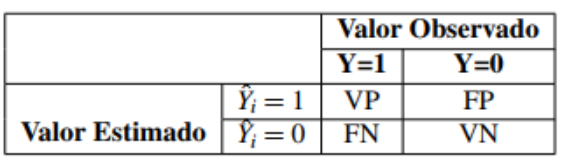
\includegraphics{matriz.png}
\caption{Matriz de Confusão}
\end{figure}

Fonte: Adaptado de FAWCETT (\protect\hyperlink{ref-Fawcett2006}{2006}).

\begin{Shaded}
\begin{Highlighting}[]
\KeywordTok{require}\NormalTok{(caret)}
\end{Highlighting}
\end{Shaded}

\begin{verbatim}
Carregando pacotes exigidos: caret
\end{verbatim}

\begin{verbatim}
Carregando pacotes exigidos: lattice
\end{verbatim}

\begin{Shaded}
\begin{Highlighting}[]
\NormalTok{  pdata <-}\StringTok{ }\KeywordTok{as.factor}\NormalTok{(}
    \KeywordTok{ifelse}\NormalTok{(}
      \KeywordTok{predict}\NormalTok{(m1, }\DataTypeTok{newdata =}\NormalTok{ chd, }\DataTypeTok{type =} \StringTok{"response"}\NormalTok{)}
      \OperatorTok{>}\FloatTok{0.5}\NormalTok{,}\StringTok{"1"}\NormalTok{,}\StringTok{"0"}\NormalTok{))}

\KeywordTok{confusionMatrix}\NormalTok{(pdata, chd}\OperatorTok{$}\NormalTok{CHD, }\DataTypeTok{positive=}\StringTok{"1"}\NormalTok{)}
\end{Highlighting}
\end{Shaded}

\begin{verbatim}
Confusion Matrix and Statistics

          Reference
Prediction  0  1
         0 45 14
         1 12 29
                                        
               Accuracy : 0.74          
                 95% CI : (0.643, 0.823)
    No Information Rate : 0.57          
    P-Value [Acc > NIR] : 0.000319      
                                        
                  Kappa : 0.467         
 Mcnemar's Test P-Value : 0.844519      
                                        
            Sensitivity : 0.674         
            Specificity : 0.789         
         Pos Pred Value : 0.707         
         Neg Pred Value : 0.763         
             Prevalence : 0.430         
         Detection Rate : 0.290         
   Detection Prevalence : 0.410         
      Balanced Accuracy : 0.732         
                                        
       'Positive' Class : 1             
                                        
\end{verbatim}

\hypertarget{curva-roc}{%
\subsection{Curva ROC}\label{curva-roc}}

A Curva ROC (Receiver Operating Characteristic Curve) associada ao
modelo logístico mensura a capacidade de predição do modelo proposto,
através das predições da sensibilidade e da especificidade.

\begin{itemize}
\tightlist
\item
  Passo 1:
\end{itemize}

\texttt{require(pROC)\ roc1=plot.roc(chd\$CHD,fitted(m1))}

\begin{itemize}
\tightlist
\item
  Passo 2:
\end{itemize}

\begin{Shaded}
\begin{Highlighting}[]
\KeywordTok{plot}\NormalTok{(roc1,}
     \DataTypeTok{print.auc=}\OtherTok{TRUE}\NormalTok{, }
     \DataTypeTok{auc.polygon=}\OtherTok{TRUE}\NormalTok{, }
     \DataTypeTok{grud=}\KeywordTok{c}\NormalTok{(}\FloatTok{0.1}\NormalTok{,}\FloatTok{0.2}\NormalTok{),}
     \DataTypeTok{grid.col=}\KeywordTok{c}\NormalTok{(}\StringTok{"green"}\NormalTok{,}\StringTok{"red"}\NormalTok{), }
     \DataTypeTok{max.auc.polygon=}\OtherTok{TRUE}\NormalTok{, }
     \DataTypeTok{auc.polygon.col=}\StringTok{"lightgreen"}\NormalTok{, }
     \DataTypeTok{print.thres=}\OtherTok{TRUE}\NormalTok{)}
\end{Highlighting}
\end{Shaded}

\begin{figure}[h]

{\centering 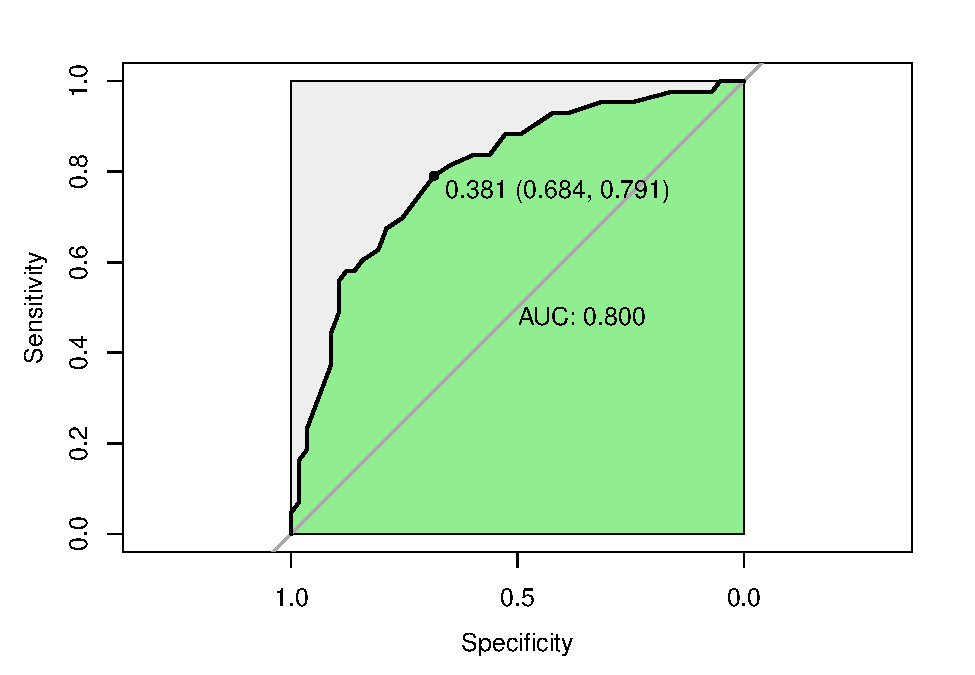
\includegraphics[width=0.6\linewidth]{05-RegLogist_files/figure-latex/roc-1} 

}

\caption{Curva Roc}\label{fig:roc}
\end{figure}

\hypertarget{o-teste-hosmer-e-lemeshow}{%
\subsection{O teste Hosmer e Lemeshow}\label{o-teste-hosmer-e-lemeshow}}

\begin{Shaded}
\begin{Highlighting}[]
\KeywordTok{require}\NormalTok{(ResourceSelection)}
\NormalTok{hl=}\KeywordTok{hoslem.test}\NormalTok{(chd}\OperatorTok{$}\NormalTok{CHD,}\KeywordTok{fitted}\NormalTok{(m1),}\DataTypeTok{g=}\DecValTok{10}\NormalTok{)}
\NormalTok{hl}
\end{Highlighting}
\end{Shaded}

\begin{verbatim}

    Hosmer and Lemeshow goodness of fit (GOF) test

data:  chd$CHD, fitted(m1)
X-squared = 100, df = 8, p-value <2e-16
\end{verbatim}

\hypertarget{pseudo-r2}{%
\subsection{Pseudo R\^{}\{2\}}\label{pseudo-r2}}

\begin{Shaded}
\begin{Highlighting}[]
\KeywordTok{require}\NormalTok{(modEvA)}
\end{Highlighting}
\end{Shaded}

\begin{verbatim}
Carregando pacotes exigidos: modEvA
\end{verbatim}

\begin{Shaded}
\begin{Highlighting}[]
\KeywordTok{RsqGLM}\NormalTok{(m1)}
\end{Highlighting}
\end{Shaded}

\begin{verbatim}
$CoxSnell
[1] 0.2541

$Nagelkerke
[1] 0.341

$McFadden
[1] 0.2145

$Tjur
[1] 0.2706

$sqPearson
[1] 0.2726
\end{verbatim}

\hypertarget{regressao-logistica-multipla}{%
\section{Regressão Logística
Múltipla}\label{regressao-logistica-multipla}}

O exemplo abaixo abordado foi extraído de TORRES-REYNA
(\protect\hyperlink{ref-Torres-Reyna2014}{2014}), onde observa-se o
banco de dados criado chamado \texttt{mydata}, possuindo as
variáveis\texttt{country},\texttt{year},\texttt{y},\texttt{y\_bin},\texttt{x1},\texttt{x2},\texttt{x3}
e\texttt{opinion}. A variável dependente é \texttt{y\_bin}, da qual foi
categorizada entre 0 e 1 conforme a ocorrência de valores negativos
em\texttt{y}. As variáveis independentes do modelo
serão\texttt{x1},\texttt{x2}e\texttt{x3}.

\begin{Shaded}
\begin{Highlighting}[]
\KeywordTok{require}\NormalTok{(foreign)}
\end{Highlighting}
\end{Shaded}

\begin{verbatim}
Carregando pacotes exigidos: foreign
\end{verbatim}

\begin{Shaded}
\begin{Highlighting}[]
\NormalTok{mydata <-}\StringTok{ }\KeywordTok{read.dta}\NormalTok{(}\StringTok{"http://dss.princeton.edu/training/Panel101.dta"}\NormalTok{) }
\KeywordTok{summary}\NormalTok{(mydata)}
\end{Highlighting}
\end{Shaded}

\begin{verbatim}
 country      year            y                 y_bin           x1        
 A:10    Min.   :1990   Min.   :-7.86e+09   Min.   :0.0   Min.   :-0.568  
 B:10    1st Qu.:1992   1st Qu.: 2.47e+08   1st Qu.:1.0   1st Qu.: 0.329  
 C:10    Median :1994   Median : 1.90e+09   Median :1.0   Median : 0.641  
 D:10    Mean   :1994   Mean   : 1.85e+09   Mean   :0.8   Mean   : 0.648  
 E:10    3rd Qu.:1997   3rd Qu.: 3.37e+09   3rd Qu.:1.0   3rd Qu.: 1.096  
 F:10    Max.   :1999   Max.   : 8.94e+09   Max.   :1.0   Max.   : 1.446  
 G:10                                                                     
       x2               x3              opinion  
 Min.   :-1.622   Min.   :-1.165   Str agree:20  
 1st Qu.:-1.216   1st Qu.:-0.079   Agree    :15  
 Median :-0.462   Median : 0.514   Disag    :19  
 Mean   : 0.134   Mean   : 0.762   Str disag:16  
 3rd Qu.: 1.608   3rd Qu.: 1.155                 
 Max.   : 2.530   Max.   : 7.169                 
                                                 
\end{verbatim}

Utiliza-se uma função para Modelos Lineares Generalizados (glm - em
inglês Generalized Linear Models), determinando a variável dependente
(y\_bin), as variáveis independentes \texttt{(x1+x2+x3)}, a base de
dados a ser utilizada \texttt{(data=mydata)} e a família dos modelos
\texttt{(family\ =\ binomial(link="logit"))}.

Abaixo os resultados da estimação do modelo utilizando o comando
\texttt{summary}. Observa-se que os valores \texttt{estimados} mostram
os coeficientes em formato logarítmo de chances. Assim, quando x3
eleva-se em 1 (uma) unidade, o log das chances esperado para x3
altera-se em 0,7512. Neste ponto, observa-se que as três variáveis
independentes possuem efeitos positivos para determinação das chances do
preditor ser igual a 1, caso contrário constariam com sinal negativo. A
coluna \(Pr(>|z|)\) traz os p-valores das variáveis indicando o teste da
hipótese nula. Como resultado a variável x3 revelou significância
estatística a 10\% (\$\textless{}\$0,10), no entanto o valor usual para
considerá-la estatísticamente significante é 5\% (0,05). Para fins de
explanação do modelo, neste trabalho, serão efetuadas as demais análises
do modelo de forma explicativa.

\begin{Shaded}
\begin{Highlighting}[]
\NormalTok{logit=}\KeywordTok{glm}\NormalTok{(y_bin}\OperatorTok{~}\NormalTok{x1}\OperatorTok{+}\NormalTok{x2}\OperatorTok{+}\NormalTok{x3, }\DataTypeTok{data=}\NormalTok{mydata, }\DataTypeTok{family =} \KeywordTok{binomial}\NormalTok{(}\DataTypeTok{link=}\StringTok{"logit"}\NormalTok{))}
\KeywordTok{summary}\NormalTok{(logit)}
\end{Highlighting}
\end{Shaded}

\begin{verbatim}

Call:
glm(formula = y_bin ~ x1 + x2 + x3, family = binomial(link = "logit"), 
    data = mydata)

Deviance Residuals: 
   Min      1Q  Median      3Q     Max  
-2.028   0.235   0.554   0.702   1.084  

Coefficients:
            Estimate Std. Error z value Pr(>|z|)  
(Intercept)    0.426      0.639    0.67    0.505  
x1             0.862      0.784    1.10    0.272  
x2             0.367      0.308    1.19    0.234  
x3             0.751      0.455    1.65    0.099 .
---
Signif. codes:  0 '***' 0.001 '**' 0.01 '*' 0.05 '.' 0.1 ' ' 1

(Dispersion parameter for binomial family taken to be 1)

    Null deviance: 70.056  on 69  degrees of freedom
Residual deviance: 65.512  on 66  degrees of freedom
AIC: 73.51

Number of Fisher Scoring iterations: 5
\end{verbatim}

\begin{Shaded}
\begin{Highlighting}[]
\KeywordTok{require}\NormalTok{(stargazer)}
\KeywordTok{stargazer}\NormalTok{(logit, }\DataTypeTok{title=}\StringTok{"Resultados"}\NormalTok{,}\DataTypeTok{type =} \StringTok{"text"}\NormalTok{)}
\end{Highlighting}
\end{Shaded}

\begin{verbatim}

Resultados
=============================================
                      Dependent variable:    
                  ---------------------------
                             y_bin           
---------------------------------------------
x1                           0.862           
                            (0.784)          
                                             
x2                           0.367           
                            (0.308)          
                                             
x3                          0.751*           
                            (0.455)          
                                             
Constant                     0.426           
                            (0.639)          
                                             
---------------------------------------------
Observations                  70             
Log Likelihood              -32.760          
Akaike Inf. Crit.           73.510           
=============================================
Note:             *p<0.1; **p<0.05; ***p<0.01
\end{verbatim}

A razão de chances (OR - odds ratio em inglês) estimada no modelo terá
de ser transformada por estar apresentada na forma logarítma conforme o
modelo de regressão logística o estima. Assim, utiliza-se o pacote
\texttt{mfx} para efetuar esta transformação para todo o modelo de forma
automatizada
\texttt{(logitor(y\_bin\textasciitilde{}x1+x2+x3,data=mydata))}:

\begin{Shaded}
\begin{Highlighting}[]
\KeywordTok{require}\NormalTok{(mfx)}
\KeywordTok{logitor}\NormalTok{(y_bin}\OperatorTok{~}\NormalTok{x1}\OperatorTok{+}\NormalTok{x2}\OperatorTok{+}\NormalTok{x3,}\DataTypeTok{data=}\NormalTok{mydata)}
\end{Highlighting}
\end{Shaded}

\begin{verbatim}
Call:
logitor(formula = y_bin ~ x1 + x2 + x3, data = mydata)

Odds Ratio:
   OddsRatio Std. Err.    z P>|z|  
x1     2.367     1.856 1.10 0.272  
x2     1.443     0.445 1.19 0.234  
x3     2.120     0.964 1.65 0.099 .
---
Signif. codes:  0 '***' 0.001 '**' 0.01 '*' 0.05 '.' 0.1 ' ' 1
\end{verbatim}

O resultado acima evidencia que para uma alteração em 1 (uma) unidade em
x3, a chance de que y seja igual a 1 aumenta em 112\% ((2,12-1)*100).
Dito de outra forma, a chance de y=1 é 2,12 vezes maior quando x3
aumenta em uma unidade (sendo que aqui mantêm-se as demais variáveis
independentes constantes).

Como visto, para cada variação unitária em x3 o log das chances varia
0,7512. É possível estimar, portanto, a alteração das chances em função
das médias dos valores de cada variável x1 e x2, e utilizar como exemplo
os valores de 1, 2 e 3 para x3, para assim alcançar os preditores do log
das chances nesta simulação, como segue abaixo:

Para facilitar a interpretação do modelo, se torna mais fácil depois de
transformado a sua exponenciação dos coeficientes logísticos utilizando
o comando \texttt{exp(coef(logit))}. Desta forma, para cada incremento
unitário em x2 e mantendo as demais variáveis constantes, conclui-se que
é 1,443 vezes provável que y seja igual a 1 em oposição a não ser (igual
a zero), ou seja, as chances aumentam em 44,30\%.

\begin{Shaded}
\begin{Highlighting}[]
\KeywordTok{exp}\NormalTok{(}\KeywordTok{coef}\NormalTok{(logit))}
\end{Highlighting}
\end{Shaded}

\begin{verbatim}
(Intercept)          x1          x2          x3 
      1.531       2.367       1.443       2.120 
\end{verbatim}

O \textbf{intervalo de confiança} do modelo pode ser exposto utilizando
o comando \texttt{confint} para os coeficientes estimados, como segue
abaixo:

\begin{Shaded}
\begin{Highlighting}[]
\KeywordTok{exp}\NormalTok{(}\KeywordTok{cbind}\NormalTok{(}\DataTypeTok{OR=}\KeywordTok{coef}\NormalTok{(logit), }\KeywordTok{confint}\NormalTok{(logit)))}
\end{Highlighting}
\end{Shaded}

\begin{verbatim}
               OR  2.5 % 97.5 %
(Intercept) 1.531 0.4387  5.625
x1          2.367 0.5129 11.675
x2          1.443 0.8041  2.738
x3          2.120 1.0039  5.719
\end{verbatim}

A partir do modelo logístico, podemos realizar \textbf{predições das
probabilidades} de se encontrar o resultado y=1 conforme visto acima.
Para isto, como exercício utilizaremos as médias das observações de cada
variável independente do modelo. Em primeiro lugar deve ser criado um
data.frame com os valores médios, como segue:

\begin{Shaded}
\begin{Highlighting}[]
\NormalTok{allmean =}\StringTok{ }\KeywordTok{data.frame}\NormalTok{(}\DataTypeTok{x1=}\KeywordTok{mean}\NormalTok{(mydata}\OperatorTok{$}\NormalTok{x1),}
                     \DataTypeTok{x2=}\KeywordTok{mean}\NormalTok{(mydata}\OperatorTok{$}\NormalTok{x2),}
                     \DataTypeTok{x3=}\KeywordTok{mean}\NormalTok{(mydata}\OperatorTok{$}\NormalTok{x3))}
\NormalTok{allmean}
\end{Highlighting}
\end{Shaded}

\begin{verbatim}
     x1     x2     x3
1 0.648 0.1339 0.7619
\end{verbatim}

Utiliza-se o comando \texttt{predict()} para predição do modelo, como
segue abaixo, informando o objeto criado com a equação do modelo
(logit), a base de dados com as condições dos valores médios (allmean) e
o tipo de teste requerido (``response'') para predizer as
probabilidades. Como resultado, o modelo informa que constando os
valores médios das variáveis independentes, obtêm-se a probabilidade de
83\% em y se constituir igual a 1.

\begin{Shaded}
\begin{Highlighting}[]
\NormalTok{allmean}\OperatorTok{$}\NormalTok{pred.prob =}\StringTok{ }\KeywordTok{predict}\NormalTok{(logit, }\DataTypeTok{newdata=}\NormalTok{allmean, }\DataTypeTok{type=}\StringTok{"response"}\NormalTok{)}
\NormalTok{allmean}
\end{Highlighting}
\end{Shaded}

\begin{verbatim}
     x1     x2     x3 pred.prob
1 0.648 0.1339 0.7619    0.8329
\end{verbatim}

\hypertarget{metodo-stepwise}{%
\subsection{Método Stepwise}\label{metodo-stepwise}}

O método Stepwise auxilia o pesquisador em selecionar as variáveis
importantes ao modelo:

\begin{Shaded}
\begin{Highlighting}[]
\KeywordTok{step}\NormalTok{(logit, }\DataTypeTok{direction =} \StringTok{'both'}\NormalTok{)}
\end{Highlighting}
\end{Shaded}

\begin{verbatim}
Start:  AIC=73.51
y_bin ~ x1 + x2 + x3

       Df Deviance  AIC
- x1    1     66.7 72.7
- x2    1     67.0 73.0
<none>        65.5 73.5
- x3    1     69.4 75.4

Step:  AIC=72.74
y_bin ~ x2 + x3

       Df Deviance  AIC
- x2    1     67.3 71.3
<none>        66.7 72.7
+ x1    1     65.5 73.5
- x3    1     70.0 74.0

Step:  AIC=71.33
y_bin ~ x3

       Df Deviance  AIC
<none>        67.3 71.3
- x3    1     70.1 72.1
+ x2    1     66.7 72.7
+ x1    1     67.0 73.0
\end{verbatim}

\begin{verbatim}

Call:  glm(formula = y_bin ~ x3, family = binomial(link = "logit"), 
    data = mydata)

Coefficients:
(Intercept)           x3  
      1.134        0.487  

Degrees of Freedom: 69 Total (i.e. Null);  68 Residual
Null Deviance:      70.1 
Residual Deviance: 67.3     AIC: 71.3
\end{verbatim}

\hypertarget{regressao-logistica-multipla-com-variavel-categorica}{%
\section{Regressão Logística Múltipla com variável
categórica}\label{regressao-logistica-multipla-com-variavel-categorica}}

Abaixo segue um exemplo com uma variável dependente categórica:

\begin{itemize}
\tightlist
\item
  \textbf{admin}: Variável dependente = 0 (não admitido) e 1 (admitido)
\item
  \textbf{Rank}: Variável independente = ranking da escola de
  proveniência do candidato
\item
  \textbf{Gre}: Variável independente = exames prévios do candidato.
\item
  \textbf{Gpa}: Variável independente = exames prévios do candidato.
\end{itemize}

\begin{Shaded}
\begin{Highlighting}[]
\KeywordTok{require}\NormalTok{(readr)}
\NormalTok{binary <-}\StringTok{ }\KeywordTok{read_csv}\NormalTok{(}\StringTok{"http://www.karlin.mff.cuni.cz/~pesta/prednasky/NMFM404/Data/binary.csv"}\NormalTok{)}

\NormalTok{binary}\OperatorTok{$}\NormalTok{rank <-}\StringTok{ }\KeywordTok{factor}\NormalTok{(binary}\OperatorTok{$}\NormalTok{rank)}
\NormalTok{mylogit <-}\StringTok{ }\KeywordTok{glm}\NormalTok{(admit }\OperatorTok{~}\StringTok{ }\NormalTok{gre }\OperatorTok{+}\StringTok{ }\NormalTok{gpa }\OperatorTok{+}\StringTok{ }\NormalTok{rank, }\DataTypeTok{data =}\NormalTok{ binary, }\DataTypeTok{family =} \KeywordTok{binomial}\NormalTok{(}\DataTypeTok{link=}\StringTok{"logit"}\NormalTok{))}
\end{Highlighting}
\end{Shaded}

\begin{Shaded}
\begin{Highlighting}[]
\KeywordTok{exp}\NormalTok{(}\KeywordTok{cbind}\NormalTok{(}\DataTypeTok{OR =} \KeywordTok{coef}\NormalTok{(mylogit), }\KeywordTok{confint}\NormalTok{(mylogit)))}
\end{Highlighting}
\end{Shaded}

\begin{verbatim}
                OR    2.5 % 97.5 %
(Intercept) 0.0185 0.001889 0.1665
gre         1.0023 1.000138 1.0044
gpa         2.2345 1.173858 4.3238
rank2       0.5089 0.272290 0.9448
rank3       0.2618 0.131642 0.5115
rank4       0.2119 0.090716 0.4707
\end{verbatim}

\hypertarget{refs}{}
\leavevmode\hypertarget{ref-Fawcett2006}{}%
FAWCETT, T. \textbf{An introduction to ROC analysis}. \emph{Pattern
Recognition Letters}, {[}s.l.{]}, 2006.

\leavevmode\hypertarget{ref-Hair2009}{}%
HAIR, J. F. et al. \textbf{Análise Multivariada de Dados}. São Paulo:
Bookman, 2009.

\leavevmode\hypertarget{ref-Hosmer2000}{}%
HOSMER, D. W.; LEMESCHOW, S. \textbf{Applied Logistic Regression}. New
York: Wiley, 2000.

\leavevmode\hypertarget{ref-Siegel2017}{}%
SIEGEL, E. \textbf{Análise Preditiva: O poder de prever quem vai clicar,
comprar, mentir ou morrer}. Rio de Janeiro: Alta Books, 2017.

\leavevmode\hypertarget{ref-Torres-Reyna2014}{}%


\end{document}
